\chapter*{Annexure B: Criteria 2 Supporting Documents}
\addcontentsline{toc}{chapter}{Annexure B: Criteria 2 Supporting Documents}
\label{app:crtieria-2}

This section provides supporting annexures required for the Criterion 2: Program Learning Outcomes (PLOs).

\setcounter{section}{0}
\renewcommand{\thesection}{B.\arabic{section}}

\section{PLO--PEO Mapping Rationale}
\label{app:criteria-2_plo-peo_mapping_rationale}
A concise rationale for the PLO--PEO mapping is given in the Table~\ref{table:plo-peo_mapping_rationale}.

\setcounter{table}{0}
\renewcommand{\thetable}{B.\arabic{table}}
{\footnotesize
\begin{longtable}{>{\raggedright\arraybackslash}p{0.30\textwidth}
                  >{\centering\arraybackslash}p{0.18\textwidth}
                  >{\raggedright\arraybackslash}p{0.45\textwidth}}
\caption{PLO--PEO Mapping Rationale}
\label{table:plo-peo_mapping_rationale}\\
\toprule
\textbf{PLO} & \textbf{Mapped PEO(s)} & \textbf{Brief Rationale} \\
\midrule
\endfirsthead
\multicolumn{3}{l}{\textit{\tablename~\thetable{} (continued)}}\\
\toprule
\textbf{PLO} & \textbf{Mapped PEO(s)} & \textbf{Brief Rationale} \\
\midrule
\endhead
\midrule
\multicolumn{3}{r}{\textit{Continued on next page}}\\
\endfoot
\bottomrule
\endlastfoot

PLO-1 Engineering Knowledge        & PEO-1 & Application of software engineering knowledge and technical foundations directly supports the development of a strong software engineering skill set. \\
\addlinespace
PLO-2 Problem Analysis             & PEO-1 & Analyzing and solving complex software engineering problems is a core aspect of professional software engineering competence. \\
\addlinespace
PLO-3 Design/Development of Solutions & PEO-1 \& PEO-2 & Designing innovative software systems and solutions demonstrates the technical expertise expected from graduates. \\
\addlinespace
PLO-4 Investigation                & PEO-1 & Research, experimentation, and data-driven investigation strengthen graduates' ability to address complex software engineering challenges. \\
\addlinespace
PLO-5 Tool Usage                   & PEO-1 & Effective use of modern software engineering tools and technologies is essential for professional software development practice. \\
\addlinespace
PLO-6 The Engineer and the World   & PEO-3 & Understanding societal, environmental, economic, and sustainability impacts supports responsible and sustainable engineering practice. \\
\addlinespace
PLO-7 Ethics                       & PEO-3 & Professional ethics, legal compliance, diversity, and inclusion are fundamental requirements for responsible software engineering practice. \\
\addlinespace
PLO-8 Individual and Collaborative Team Work & PEO-2 & Teamwork and leadership capabilities enable graduates to contribute effectively and lead diverse software development teams. \\
\addlinespace
PLO-9 Communication                & PEO-2 & Effective communication is critical for collaboration, stakeholder engagement, and leadership in software engineering projects. \\
\addlinespace
PLO-10 Project Management and Finance & PEO-2 & Project planning, resource management, and leadership skills support successful management of software engineering projects. \\
\addlinespace
PLO-11 Lifelong Learning           & PEO-1 & Continuous learning and adaptability enable graduates to maintain and enhance their software engineering knowledge and skills throughout their careers. \\
\bottomrule
%\end{tabular}
\label{table:plo-peo_mapping_rationale}
\end{longtable}

%\section{Sample Course Outline}
%\label{Sample Course Outline}
%A sample course outline of CS251-Design and Analysis of Algorithms is attached for reference.

%\includefullannexure{appendices/criterion_2/CS-251 Design and Analysis of Algorithms Spring 2026.pdf}


%\begin{landscape}

\section{OBE Assessment Configuration and CLO--PLO Attainment through Qalam}
\label{OBE Assessment Configuration on Qalam}
This section discusses how assessments are created and mapped on different CLOs. Figure~\ref{figure:CLO-PLO mapping of sample course} shows CLO-PLO mapping of CS-251 Design and Analysis of Algorithms, a sample course, where CLOs 1, 2 and 3 are mapped to PLOs 2, 3 and 4, respectively. This CLO-PLO mapping is set by LQEC using the DLQEC account on Qalam.

\setcounter{figure}{0}
\renewcommand{\thefigure}{B.\arabic{figure}}

\begin{figure}[h]
\centering
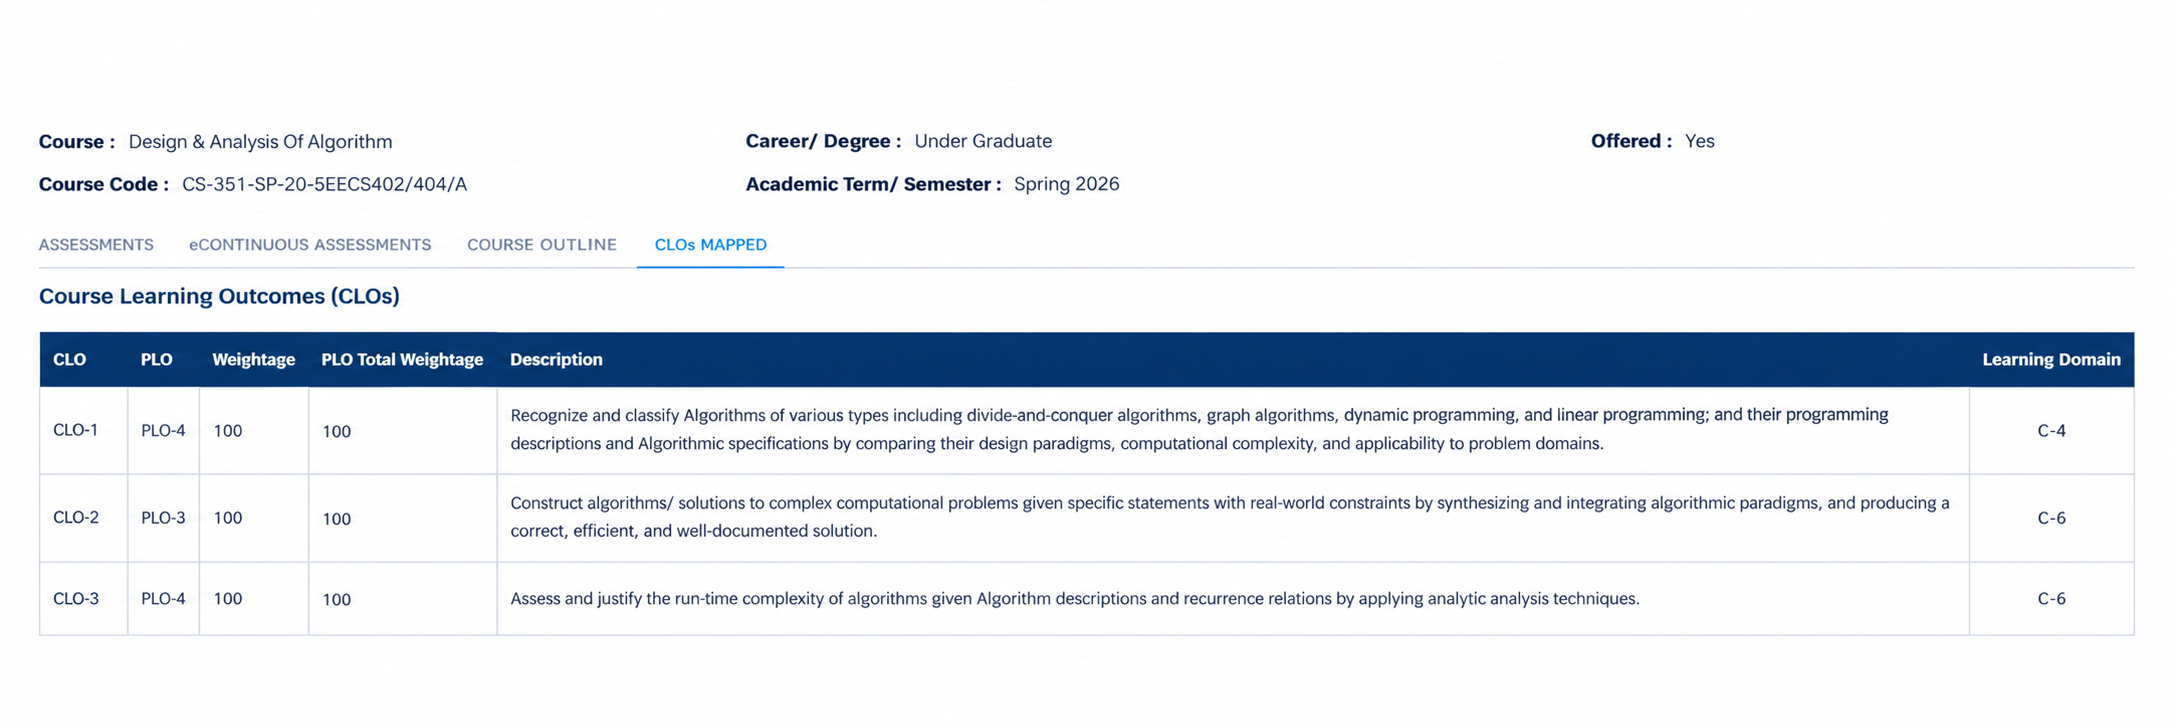
\includegraphics[width=1.0\textwidth]{images/criterion_2/media/image-7.png}
\caption{CLO-PLO Mapping of CS-251 Design and Analysis of Algorithms}
\label{figure:CLO-PLO mapping of sample course}
\end{figure}

In step 2, the total marks and weightage for each assessment are set. Then, each assessment is mapped to a pertinent CLOs with appropriate CLO weightage as shown in Figure~\ref{figure:assessments showing on qalam}. 

\begin{figure}[H]
\centering
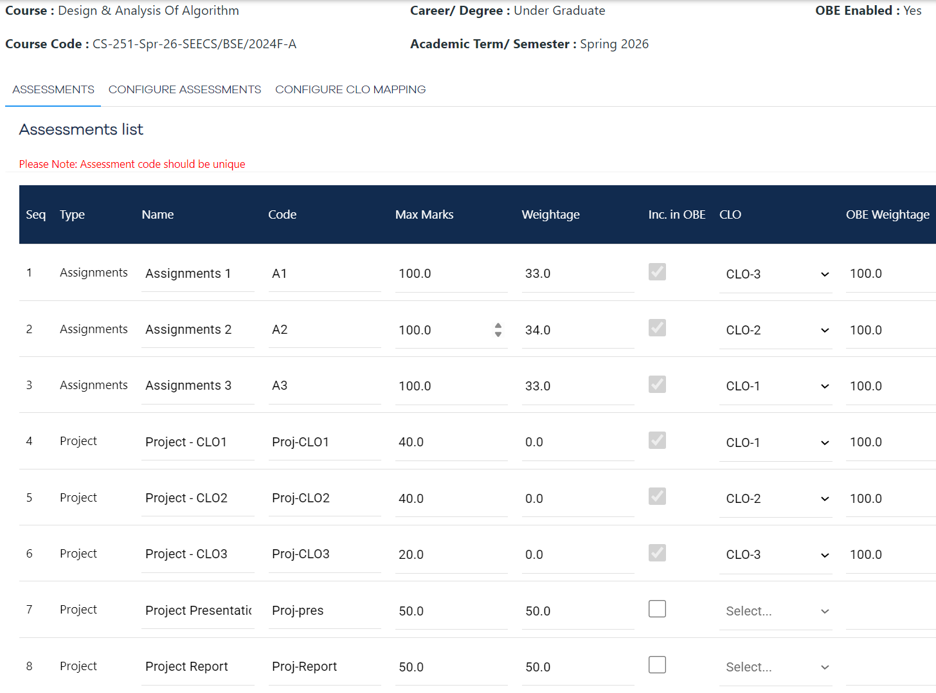
\includegraphics[width=1.0\textwidth]{images/criterion_2/media/image8.png}
\caption{Snippet of Qalam Result Section Showing Number of Assessments, their Total Marks, Weightage, and Mapping to Appropriate CLO along with the CLO Weightages}
\label{figure:assessments showing on qalam}
\end{figure}

Multiple assignments, quizes, and Mid \& End Semester Exams have been created among others. The weightage of each assessment is also set for the calculation of aggregate percentage of the course. The assessment is enabled as an OBE assessment that means the marks obtained in these assessments will be used to calculate the CLO attainment score. Appropriate CLO is mapped to each assessment, and CLO weightage is also defined (100 weightage means that each assessment has an equal weightage during CLO attainment calculations).
%\end{landscape}

After configuring the assessments, the marks obtained for each assessment are entered manually by the instructor. Once the data is entered, the result will be compiled by Qalam. The compiled result is also visible to the students. Each instructor can download the CLO and PLO attainment reports of his/her course. Annexure~\ref{Sample CLO Attainment Report} shows the CLO attainment report of CS-251 Design and Analysis of Algorithms course that highlights the CLO attainment in green and CLO not attained in red for each student. Attainment score for each CLO is also visible. The percentage CLO attainment for individuals and cohorts is then calculated. Based on the CLOs the mapped PLOs are evaluated as well in terms of `Yes' or `No' as per the defined KPIs. Annexure~\ref{Sample PLO Attainment Report} shows PLOs score and attainment for the CS-251 Design and Analysis of Algorithms course for 2024 batch.

\section{Sample CLO Attainment Report}
\label{Sample CLO Attainment Report}
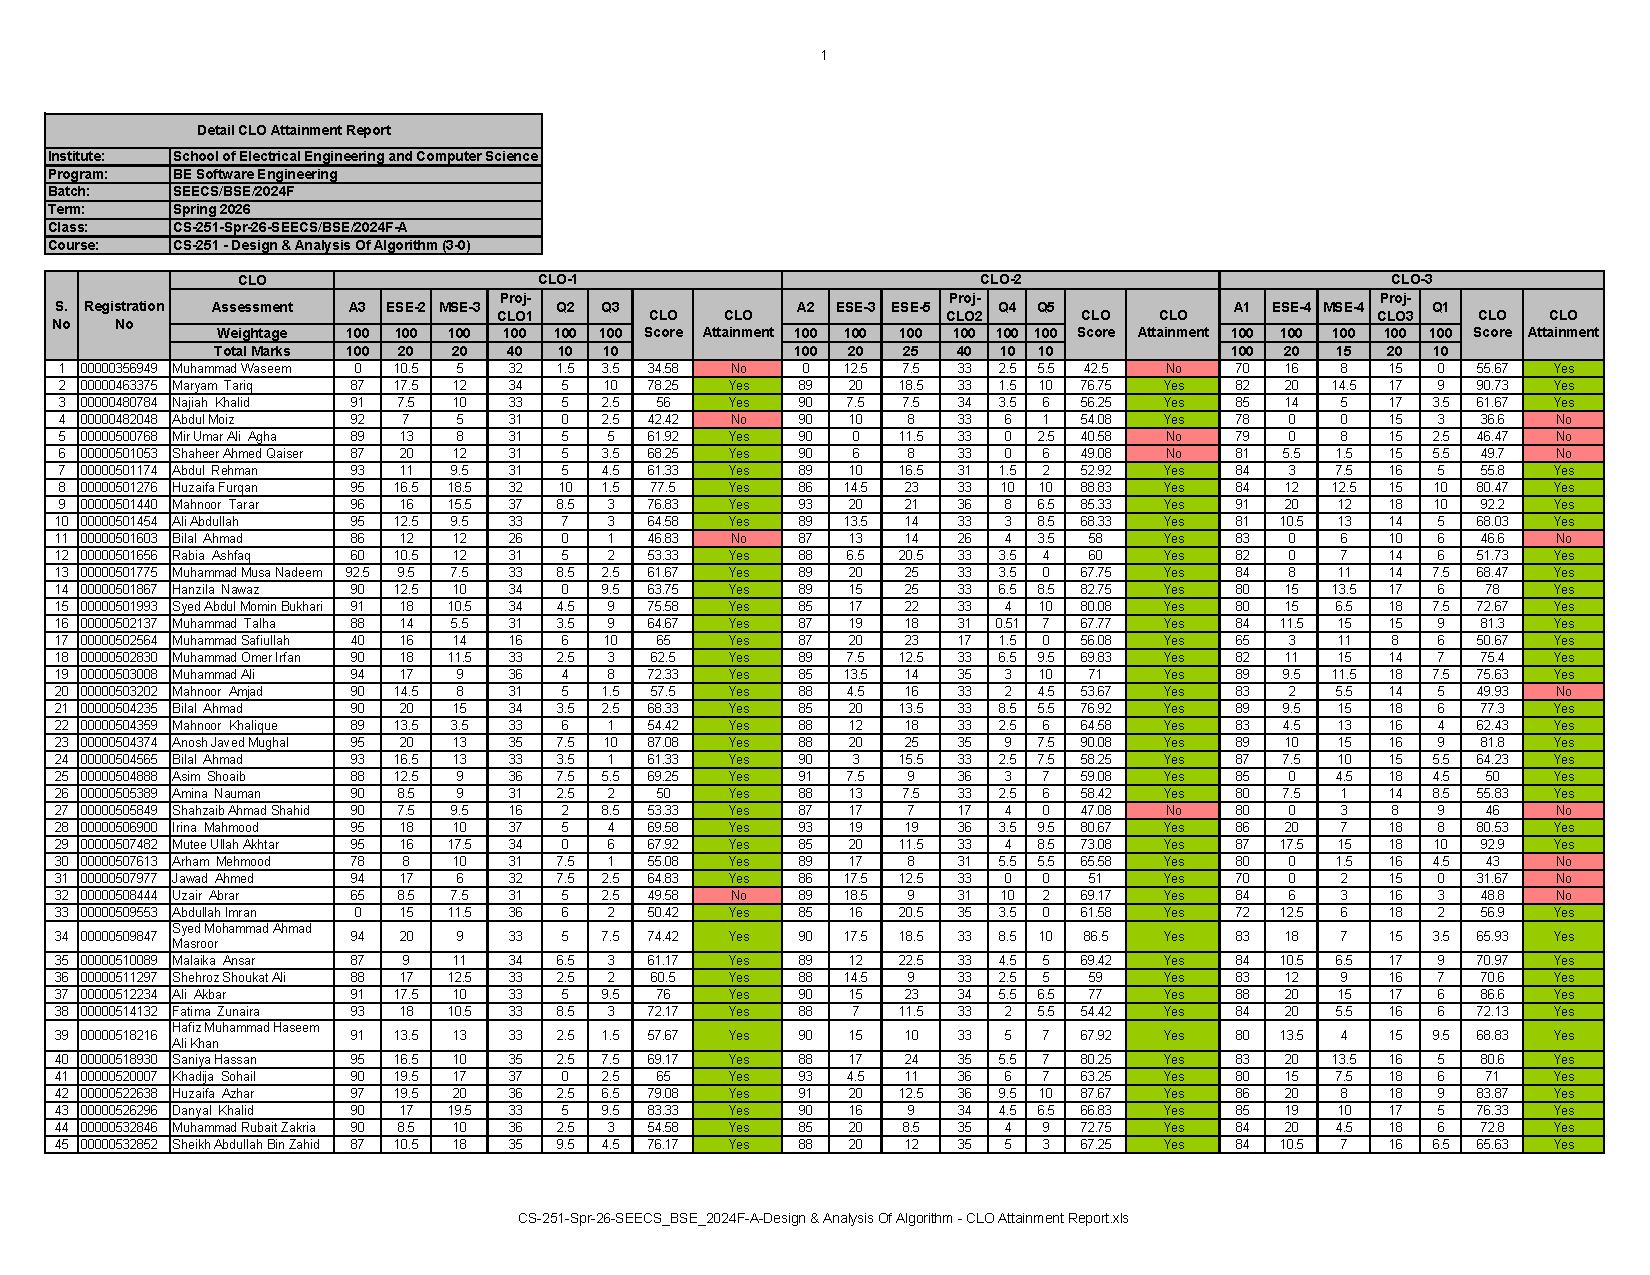
\includepdf[
    pages=-,
    landscape,
    fitpaper=true
]{appendices/criterion_2/Sample CLO Attainment Report.pdf}

\section{Sample PLO Attainment Report}
\label{Sample PLO Attainment Report}
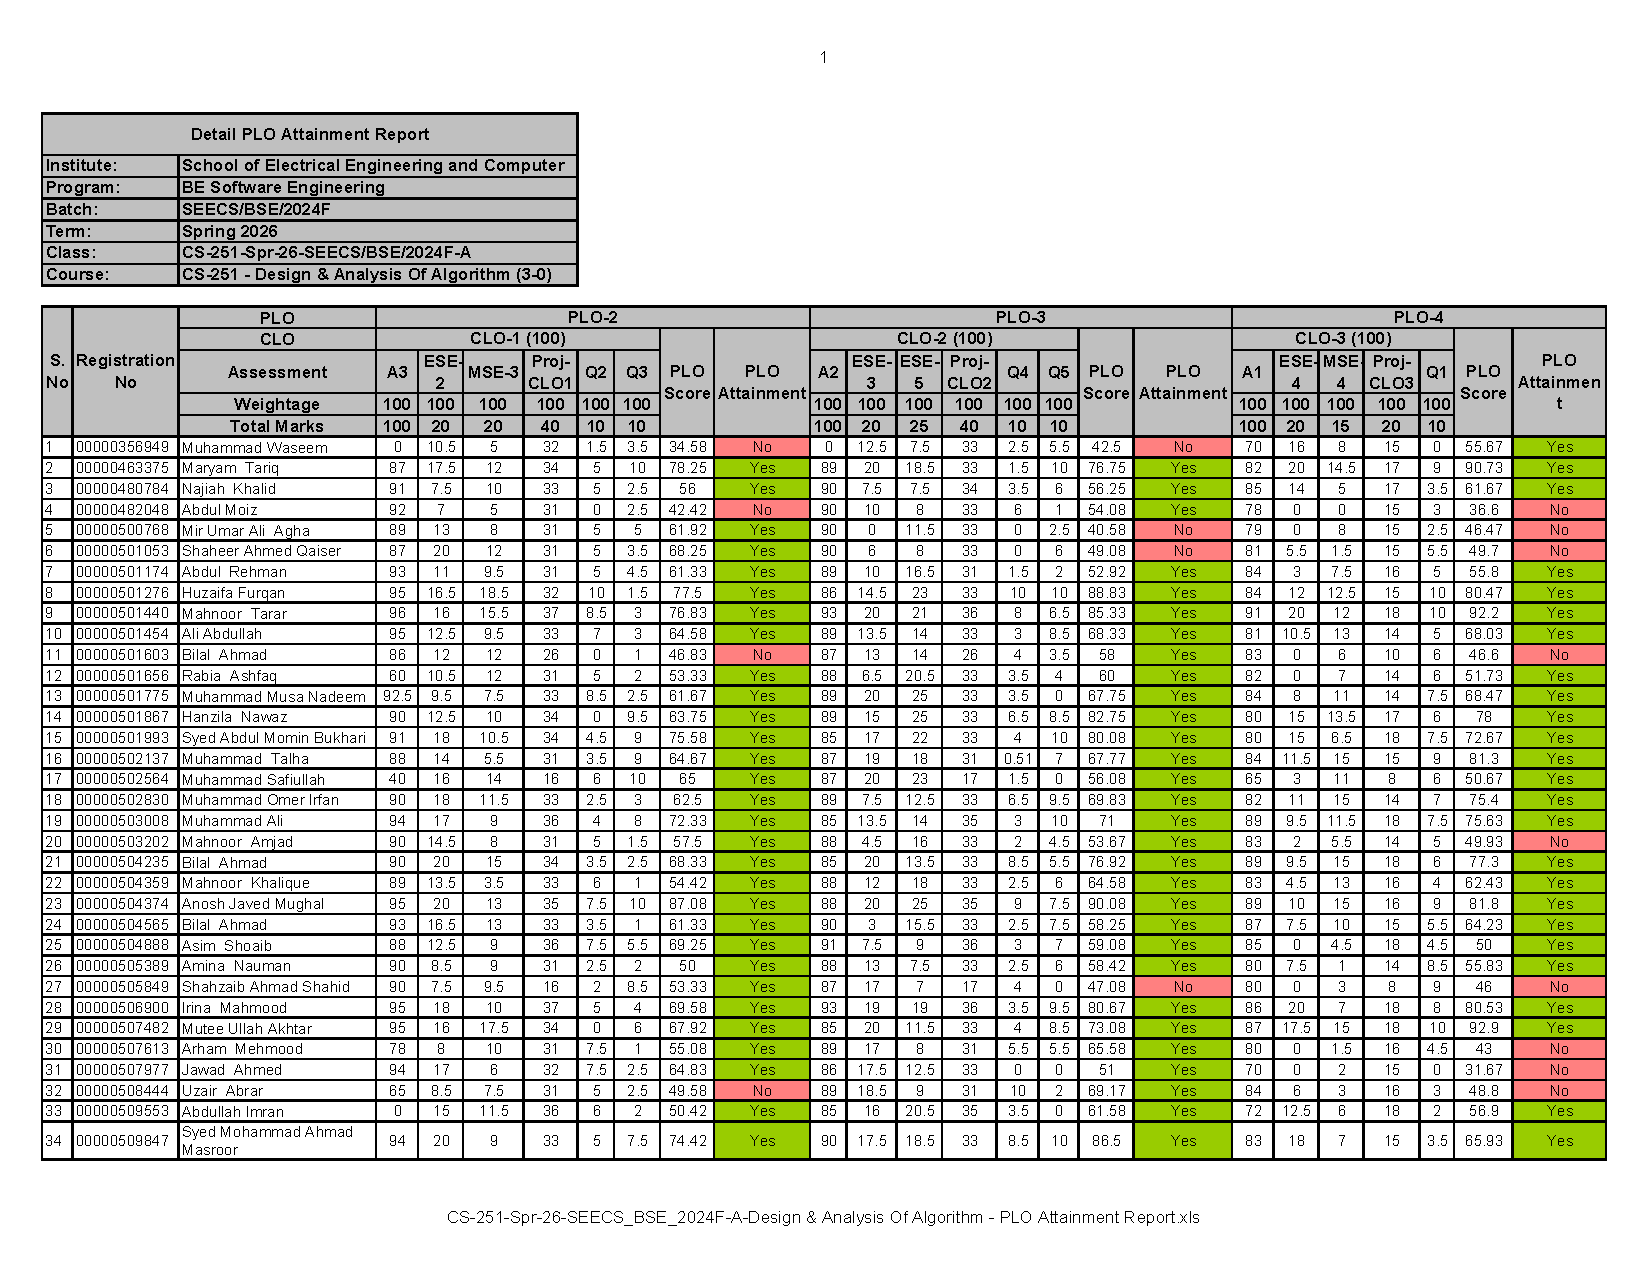
\includepdf[
   pages=-,
    landscape,
    fitpaper=true
]{appendices/criterion_2/Sample PLO Attainment Report.pdf}

\section{Consolidated PLO Attainment Report of 2K22 batch after Fall 2025 (7th Semester)}
\label{Consolidated PLO Attainment Report}
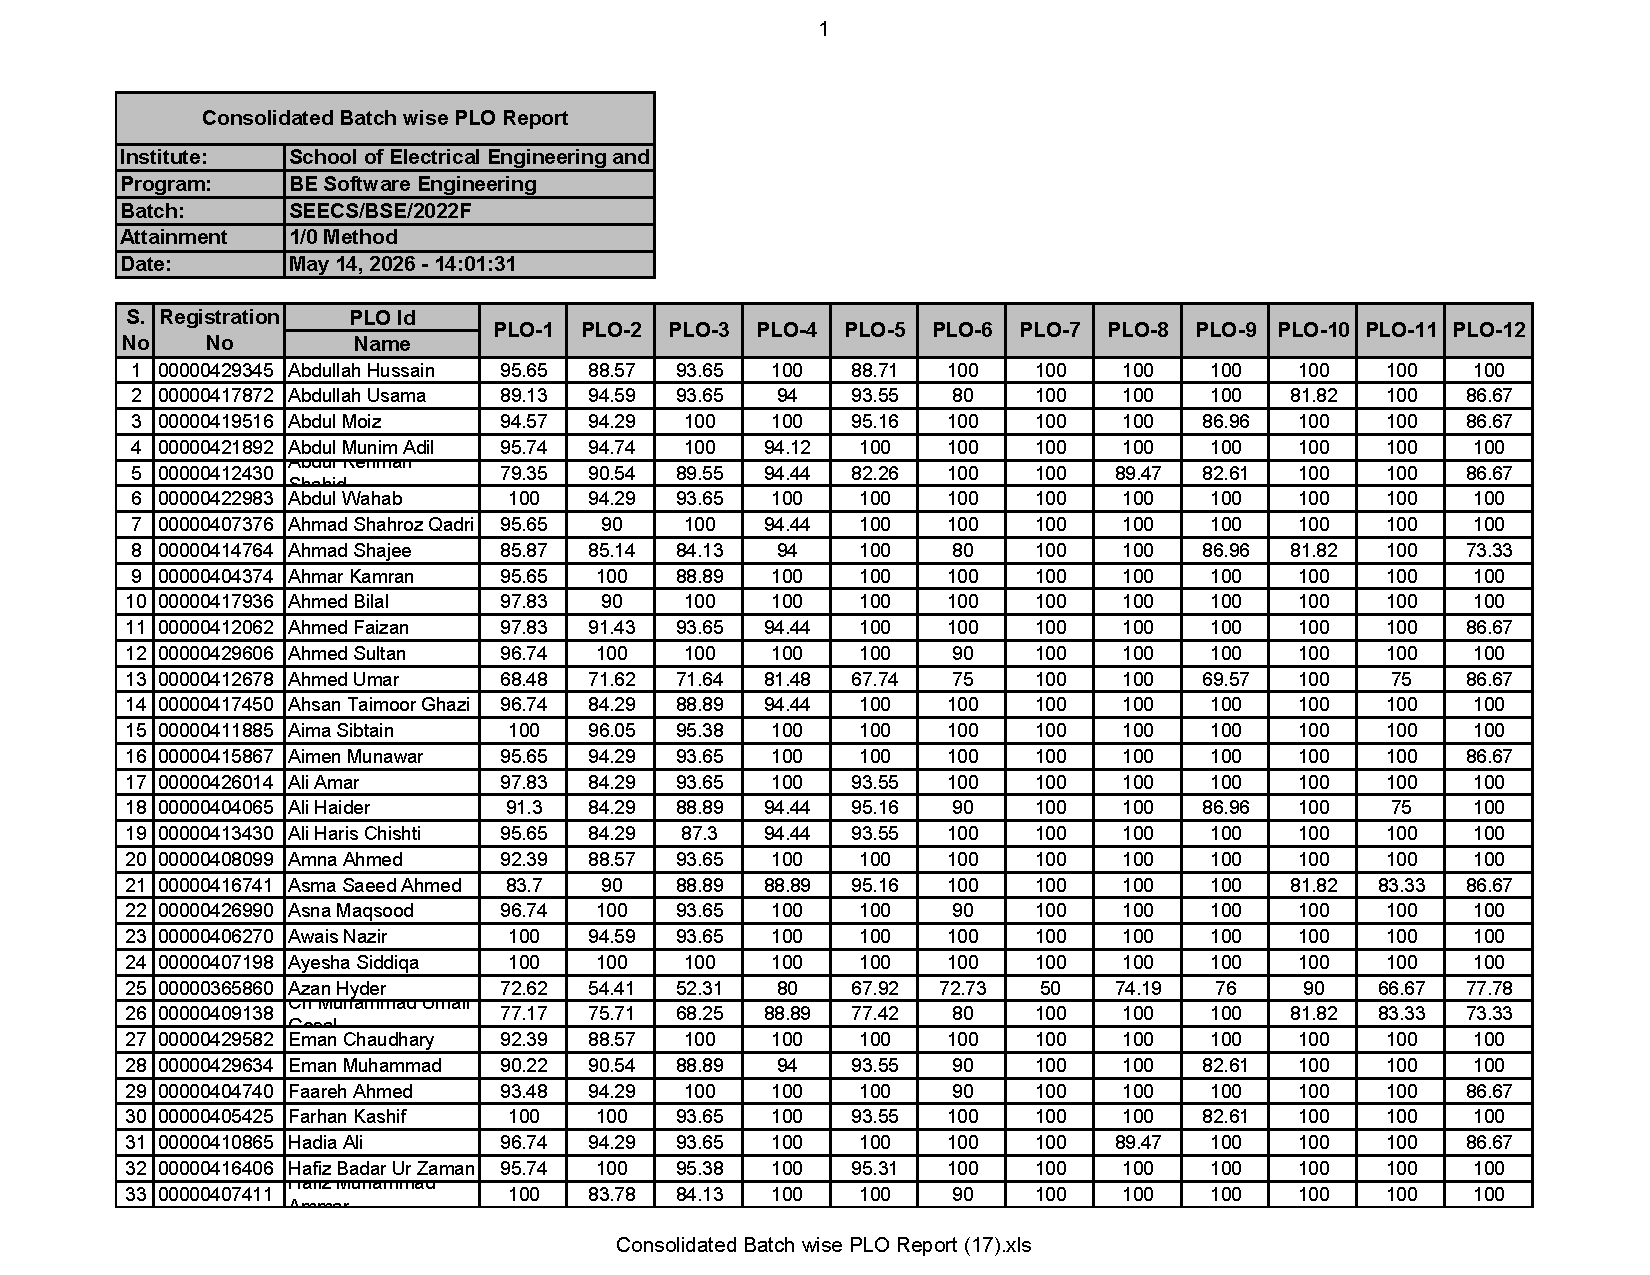
\includepdf[
    pages=-,
    landscape,
    fitpaper=true
]{appendices/criterion_2/Consolidated Batch wise PLO Report.pdf}



\clearpage
\section{CLO-PLO Attainment Results for Fall 2025 Semester}
\label{annex:clo-plo-attainment-results}
This section discusses the CLO-PLO attainment results of intake 2K22, 2K24 and 2K25 batches for Fall 2025 semester. The following subsections provides detail analysis for CLO-PLO attainment.

\subsection{2K22 Batch Fall 2025 Semester Results}

Figure~\ref{figure:2K22-batch-clo-plo-results} shows a screenshot of spreadsheet for all the courses taken by 2K22 batch in Fall 2025 semester. The figure contains CLO-PLO mapping and percentage of CLO attainment that is directly imported from the individual CLO and PLO attainment reports of each course from Qalam. Figure~\ref{figure:2022 Batch cohort CLO attainment} shows same information as bar chart showing percentage attainment of corresponding CLOs against each course. Figure~\ref{figure:2022 Batch cohort CLO attainment} also shows calculation of PLOs attainment as ``Ys'' as well as in percentage. The same information is given for PLO percentages and overall batch PLO attainment percentage in Figure~\ref{figure:2022 Batch course-wise PLO attainment} and Figure~\ref{figure:2022 Batch cohort PLO attainment}, respectively. It can be seen that the cohort has successfully attained the concerned CLOs for each course. Similarly, the cohort PLOs have been attained as per set KPIs.

\begin{figure}[H]
\centering
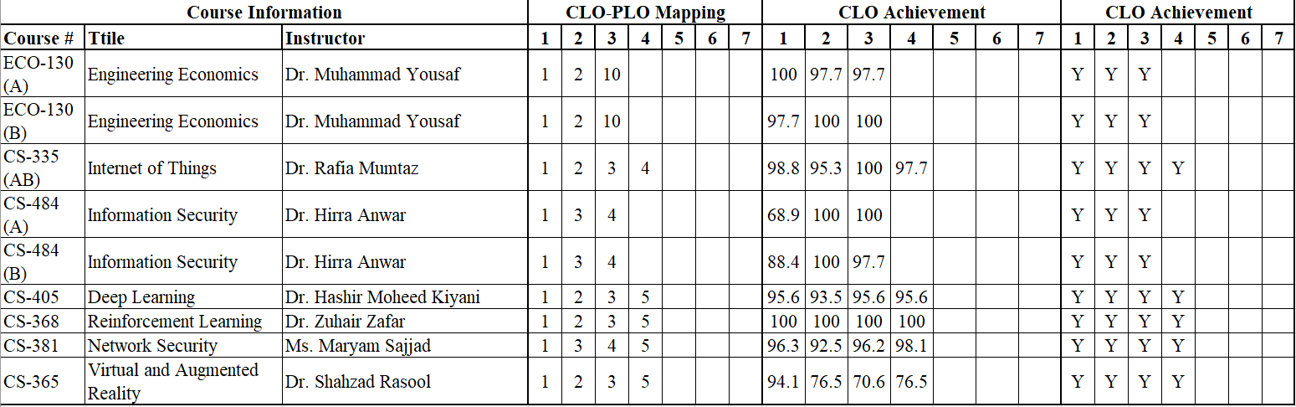
\includegraphics[width=0.98\linewidth]{images/criterion_2/media/image13.png}
\par\medskip
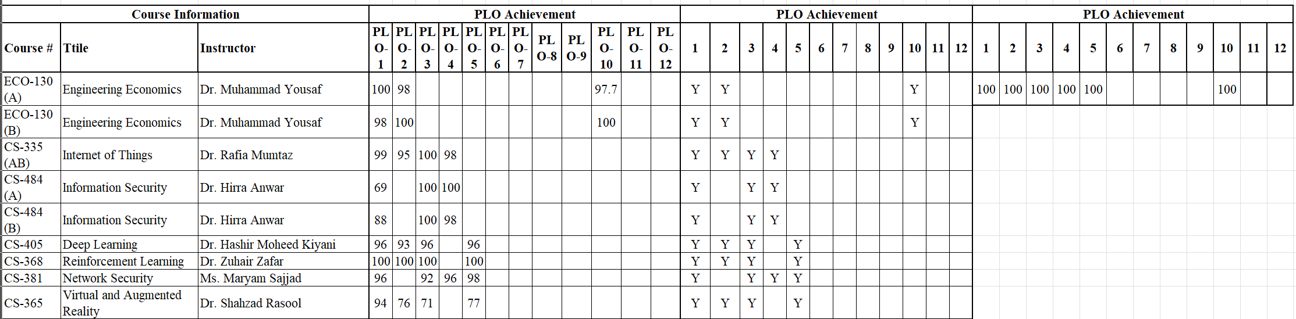
\includegraphics[width=0.98\linewidth]{images/criterion_2/media/image14.png}
\caption{ 2K22 Batch Result for All Courses in Fall 2025 Semester}
\label{figure:2K22-batch-clo-plo-results}
\end{figure}

\begin{figure}[H]
\centering
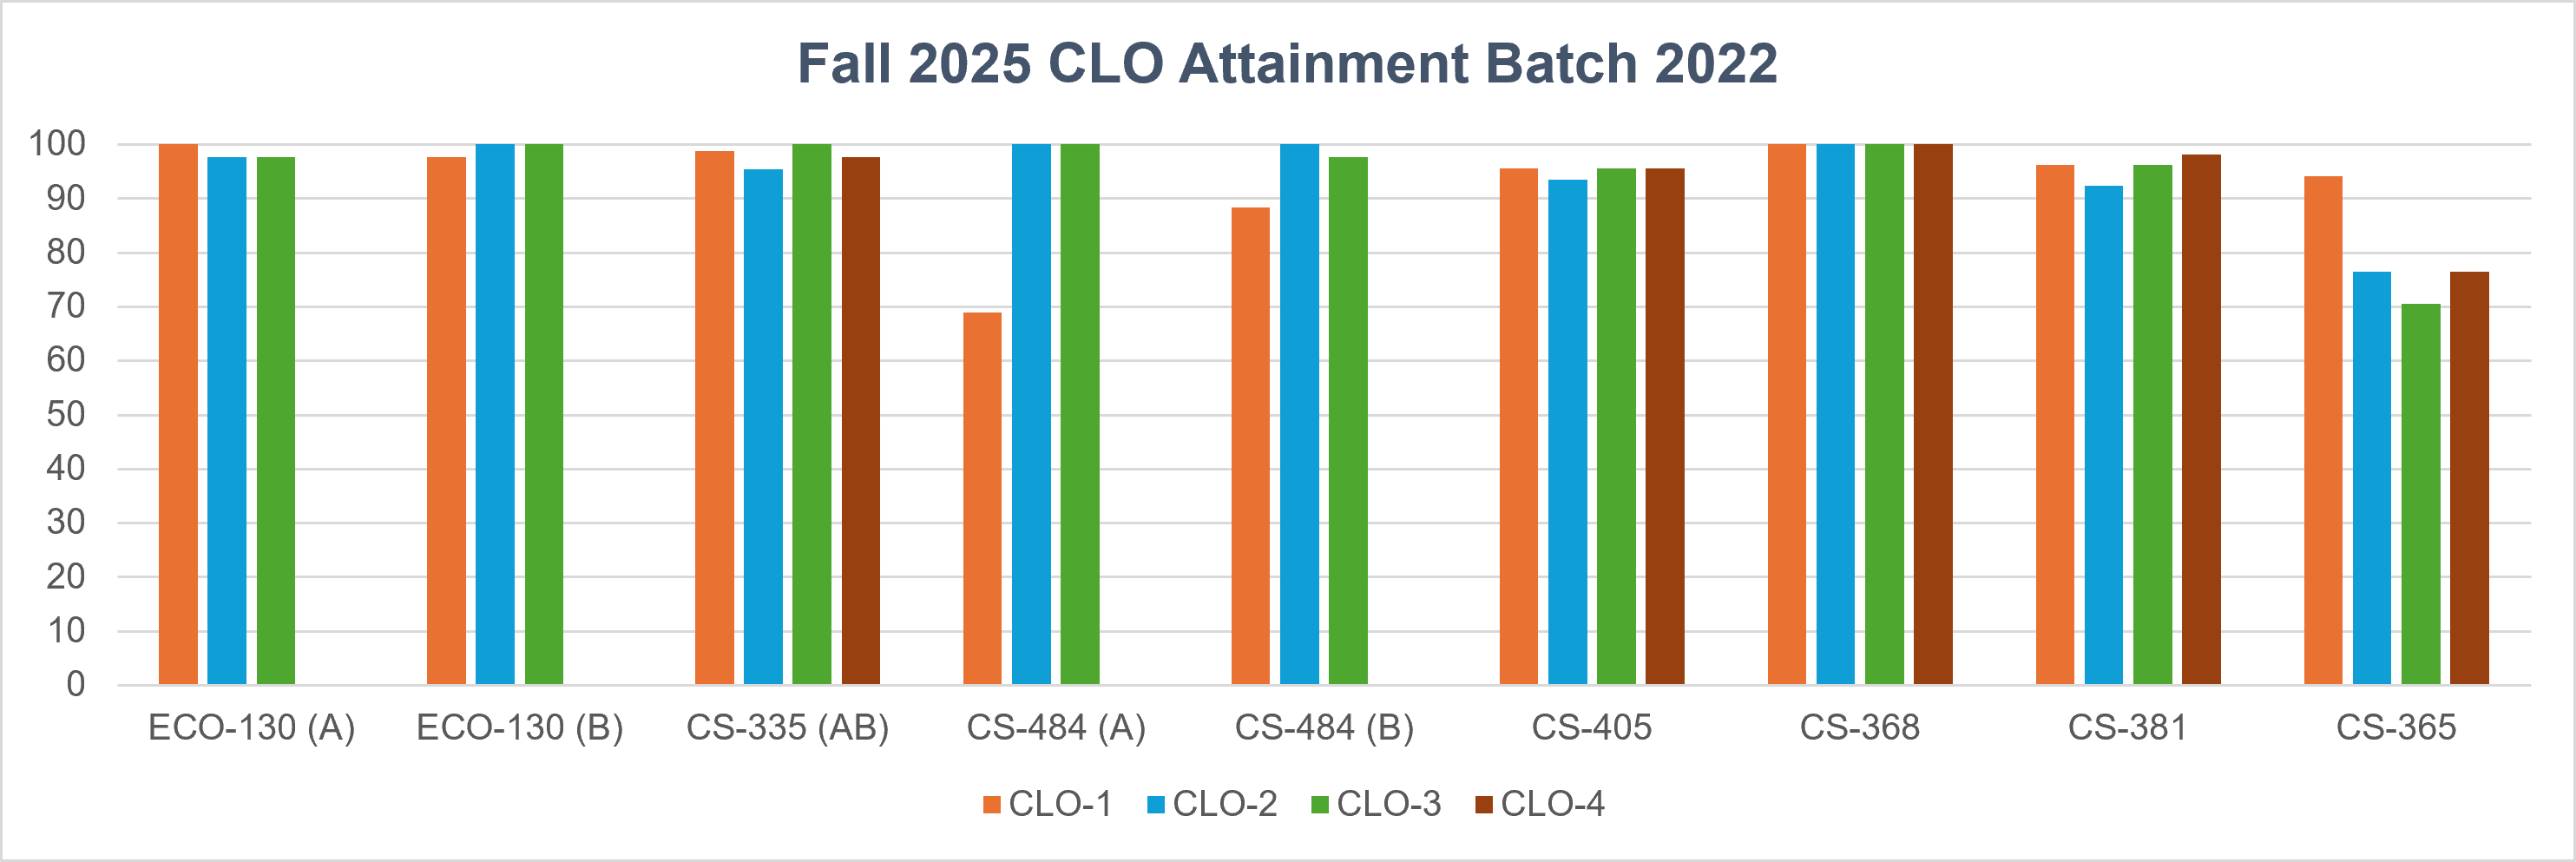
\includegraphics[width=0.95\textwidth]{images/criterion_2/media/image23.png}
\caption{2K22 Batch cohort CLO attainment for all courses in Fall 2025.}
\label{figure:2022 Batch cohort CLO attainment}
\end{figure}

\begin{figure}[H]
\centering
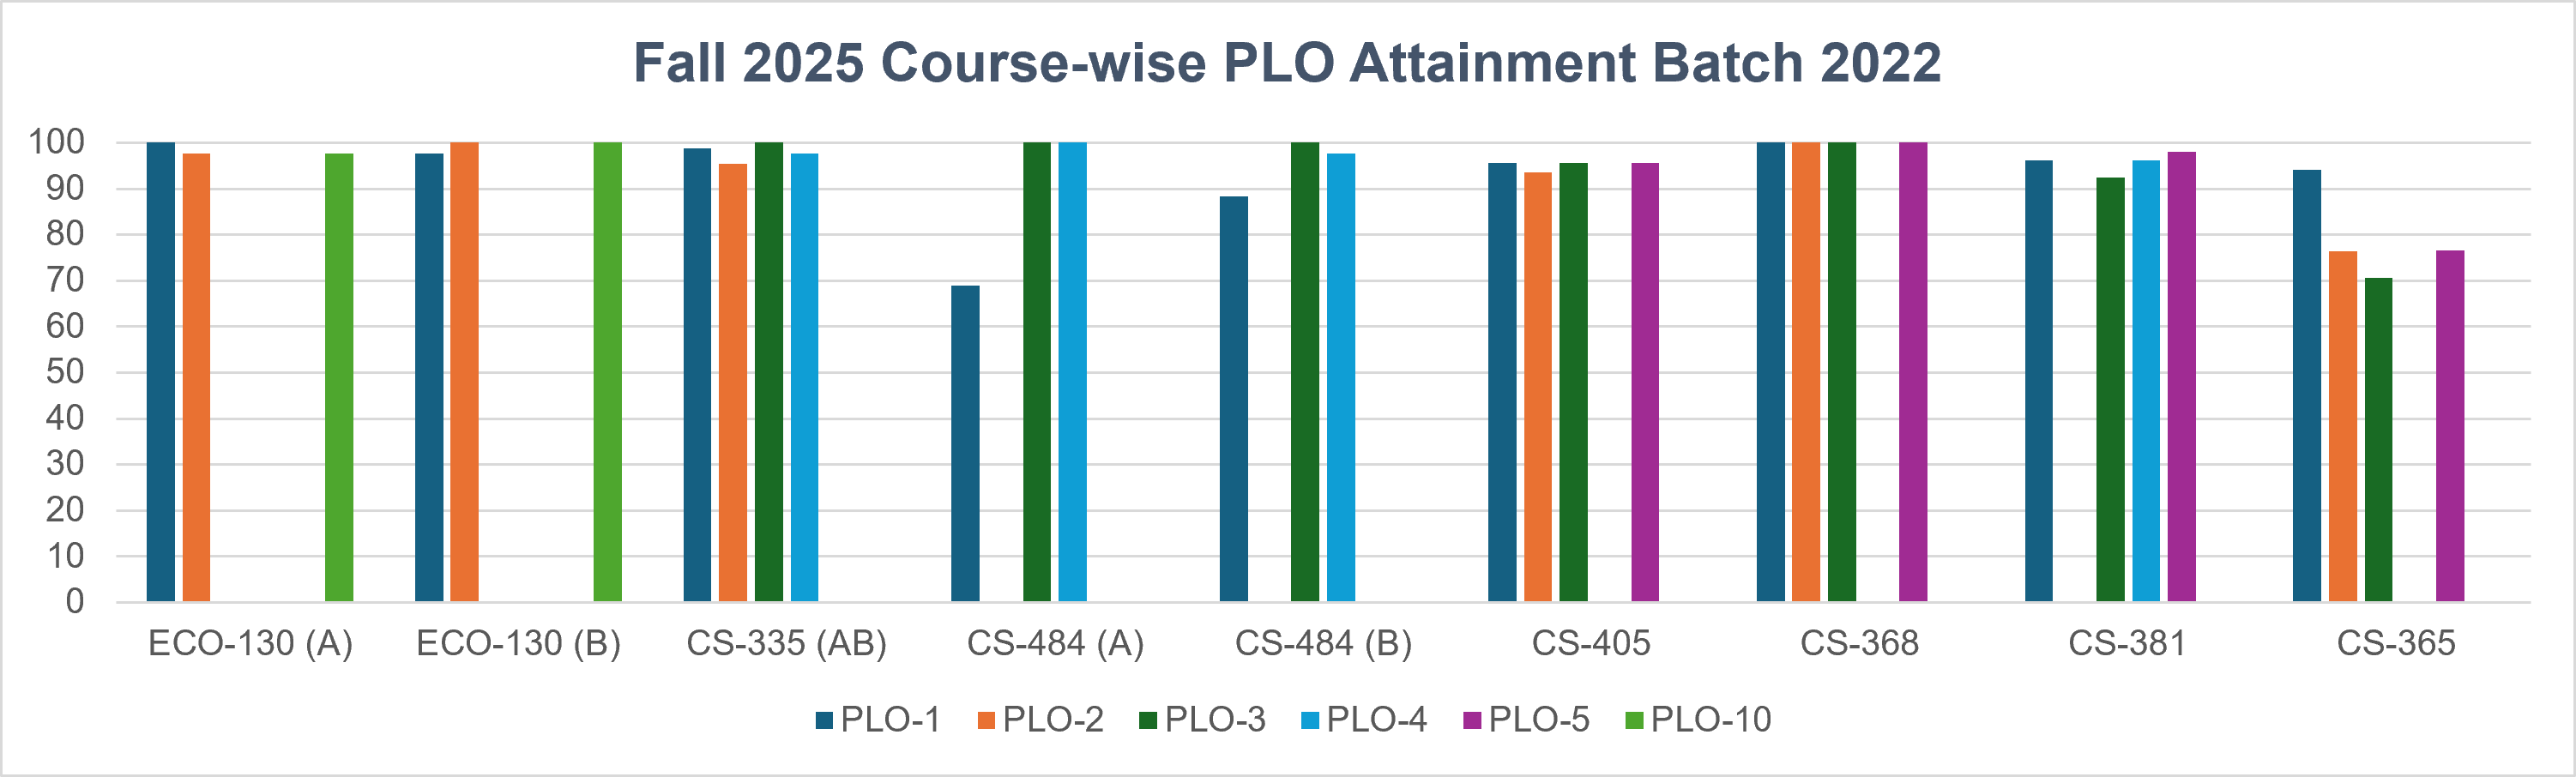
\includegraphics[width=0.95\textwidth]{images/criterion_2/media/image24.png}
\caption{2K22 Batch course-wise PLO attainment for Fall 2025.}
\label{figure:2022 Batch course-wise PLO attainment}
\end{figure}

\begin{figure}[H]
\centering
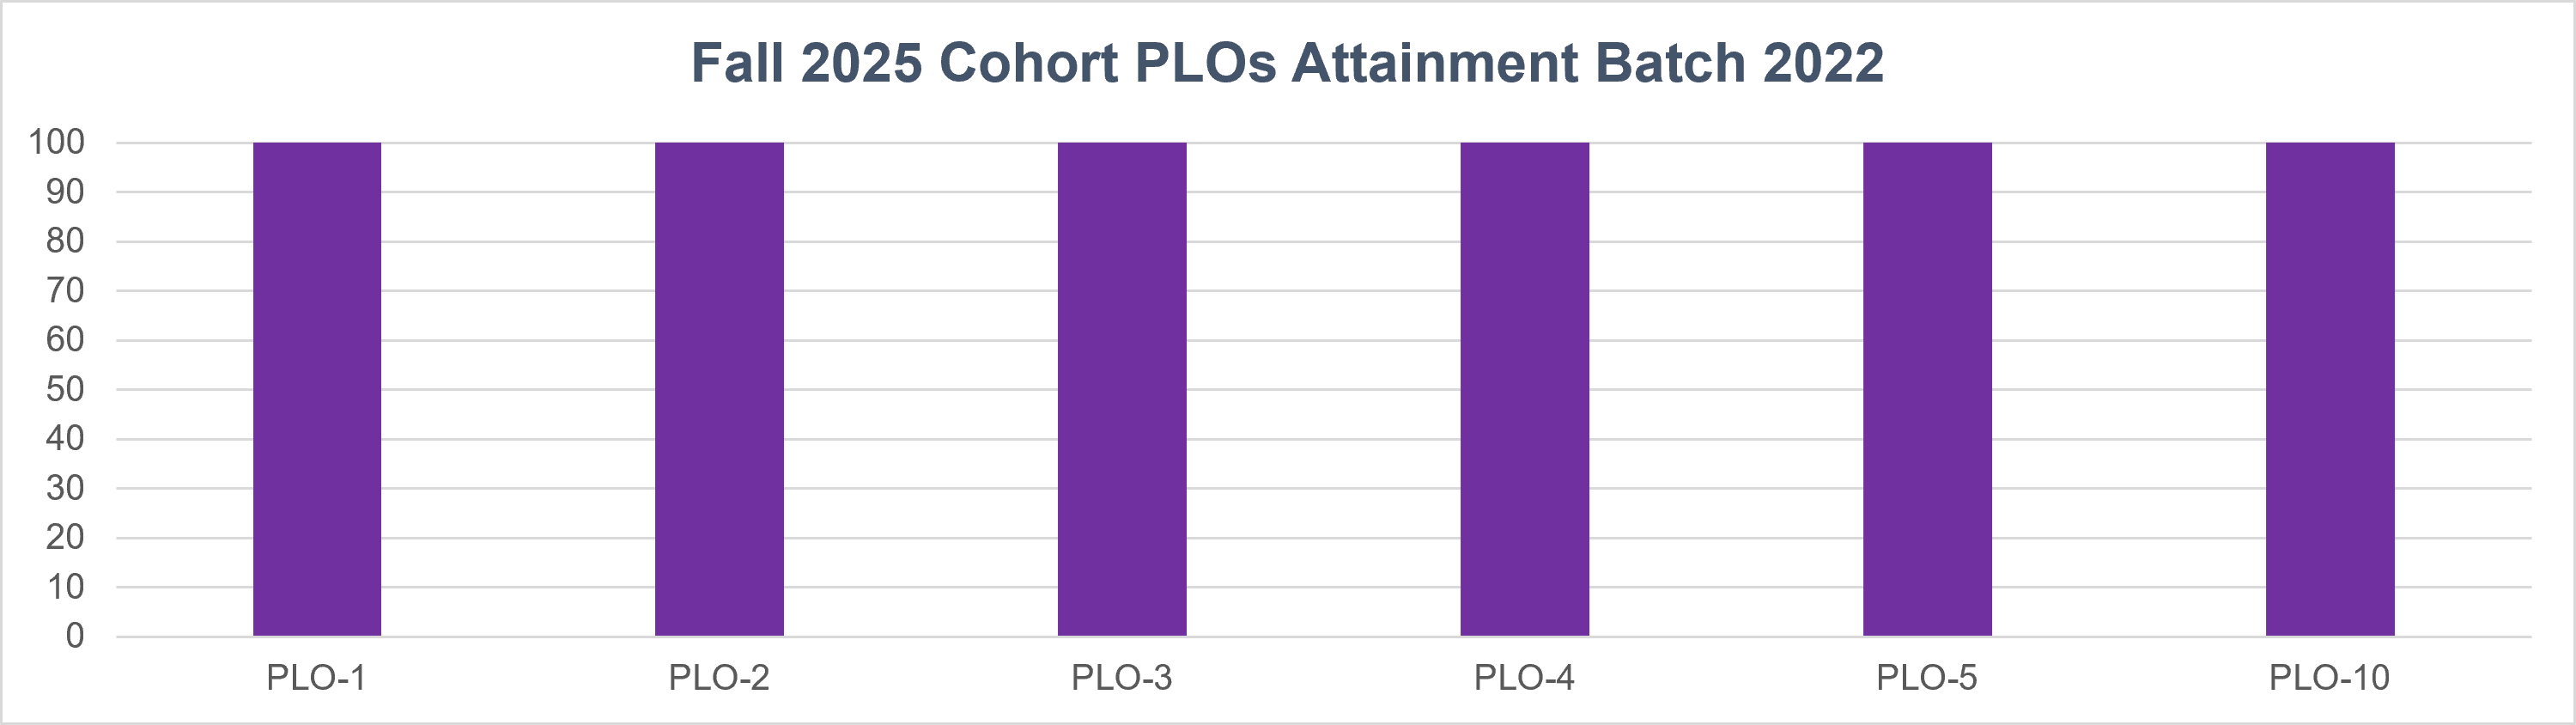
\includegraphics[width=0.95\textwidth]{images/criterion_2/media/image25.png}
\caption{2K22 Batch cohort PLO attainment against the 60\% KPI.}
\label{figure:2022 Batch cohort PLO attainment}
\end{figure}

\subsection{2K24 Batch Fall 2025 Semester Results}

The results for 2K24 batch are given in Figure~\ref{figure:2024 Batch Result for All Courses} to Figure~\ref{figure:2024 Batch cohort PLO attainment against}. It can be seen that the 2K24 batch has attained the assessed CLOs as well as the mapped PLOs on cohort level as per the set KPIs.

\begin{figure}[H]
\centering
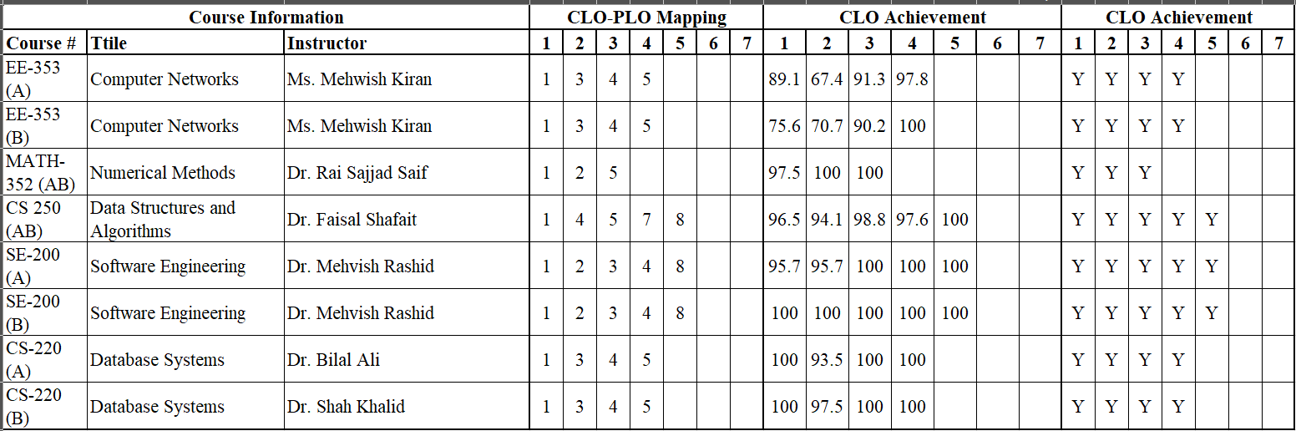
\includegraphics[width=0.98\linewidth]{images/criterion_2/media/image26.png}
\par\medskip
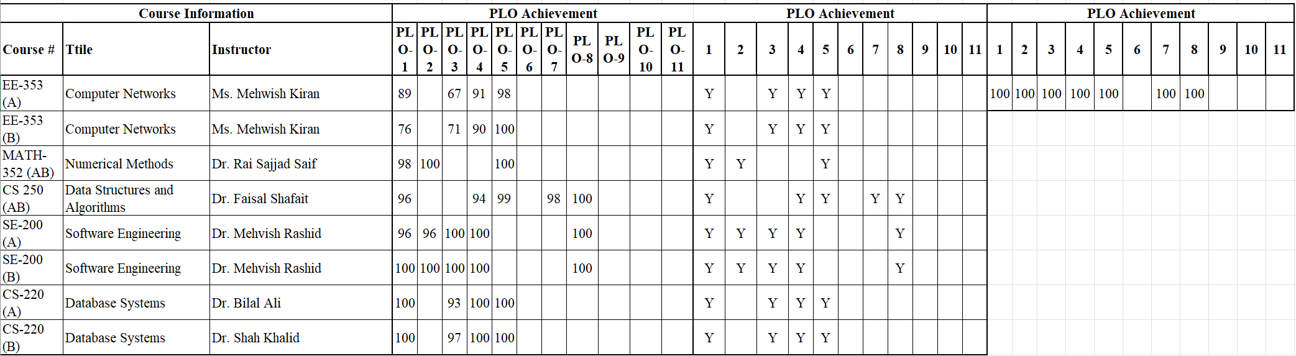
\includegraphics[width=0.98\linewidth]{images/criterion_2/media/image27.png}
\caption{2K24 Batch Result for All Courses in Fall 2025 Semester}
\label{figure:2024 Batch Result for All Courses}
\end{figure}

\begin{figure}[H]
\centering
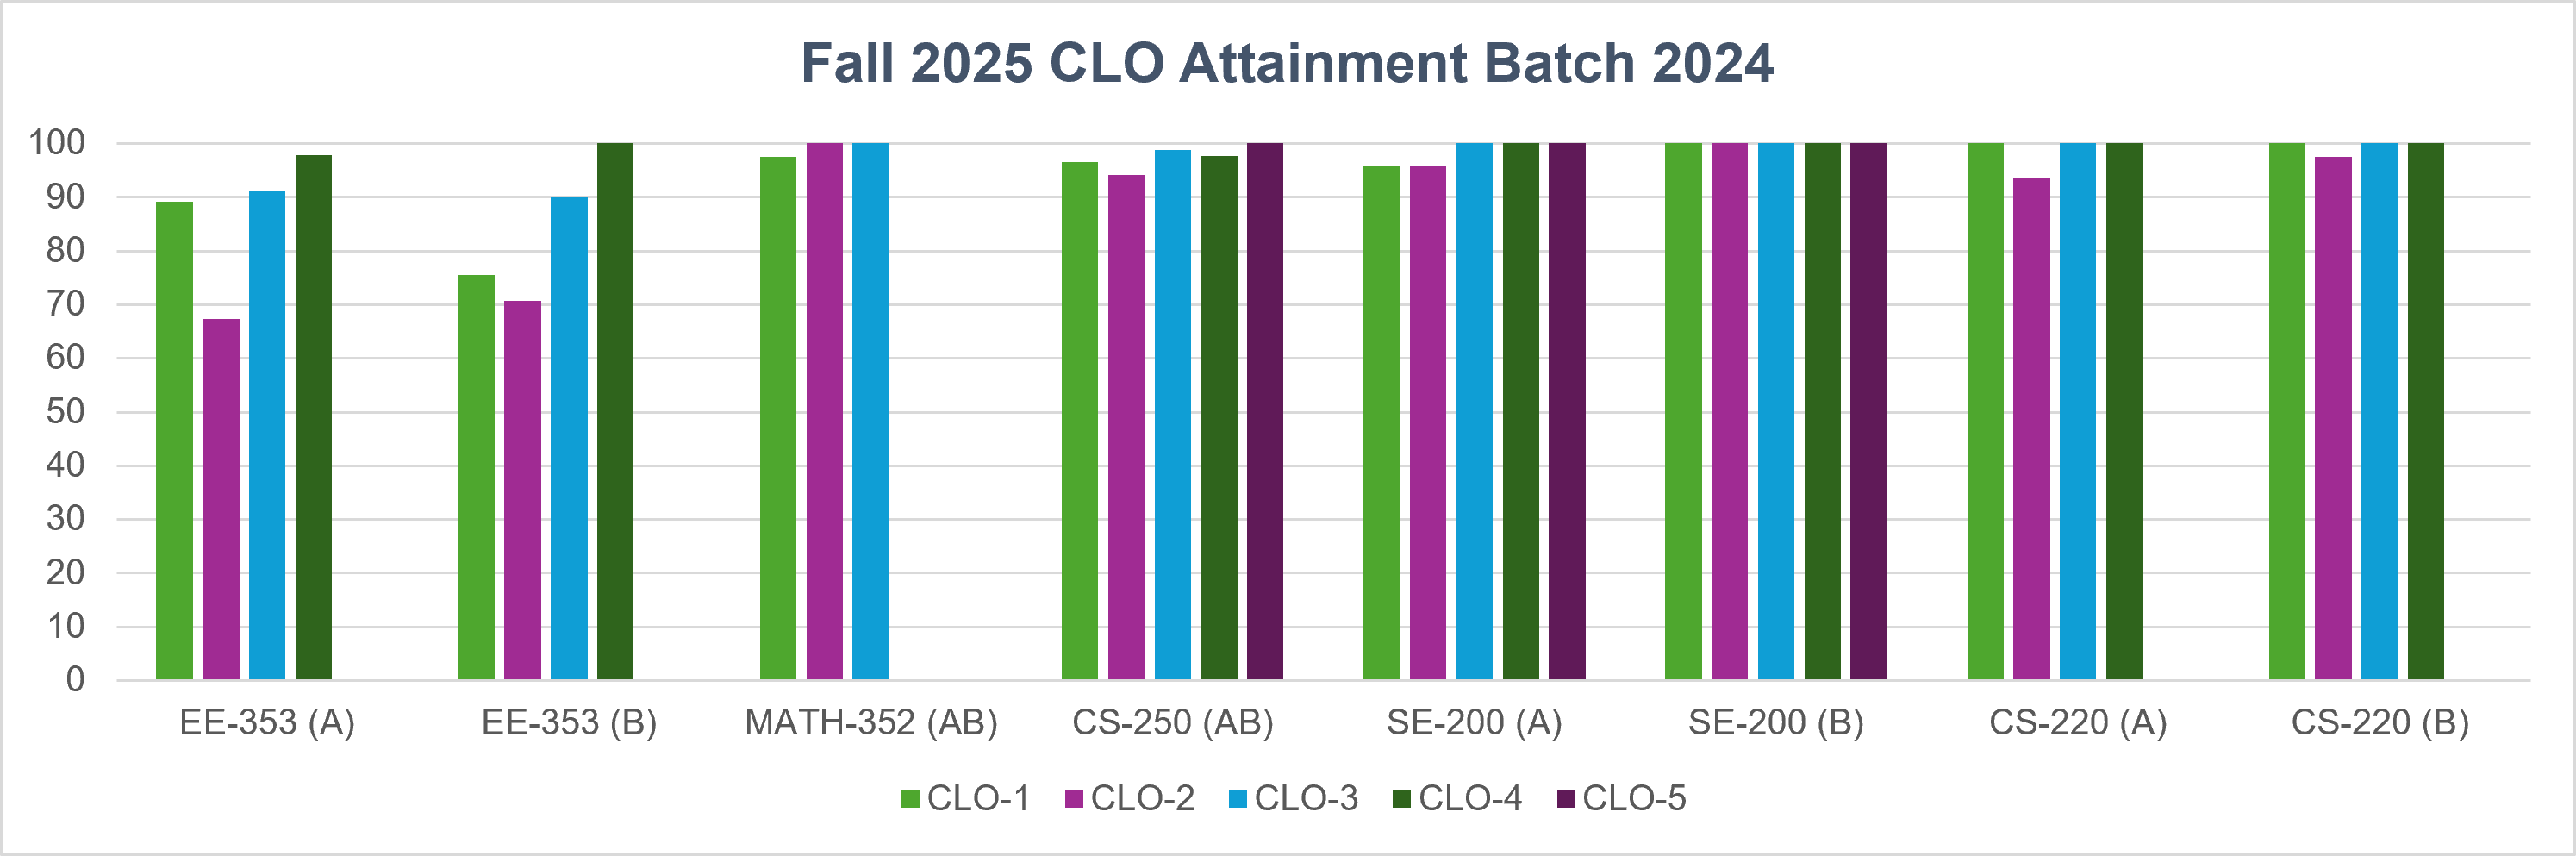
\includegraphics[width=0.95\textwidth]{images/criterion_2/media/image28.png}
\caption{2K24 Batch cohort CLO attainment for all courses in Fall 2025.}
\end{figure}

\begin{figure}[H]
\centering
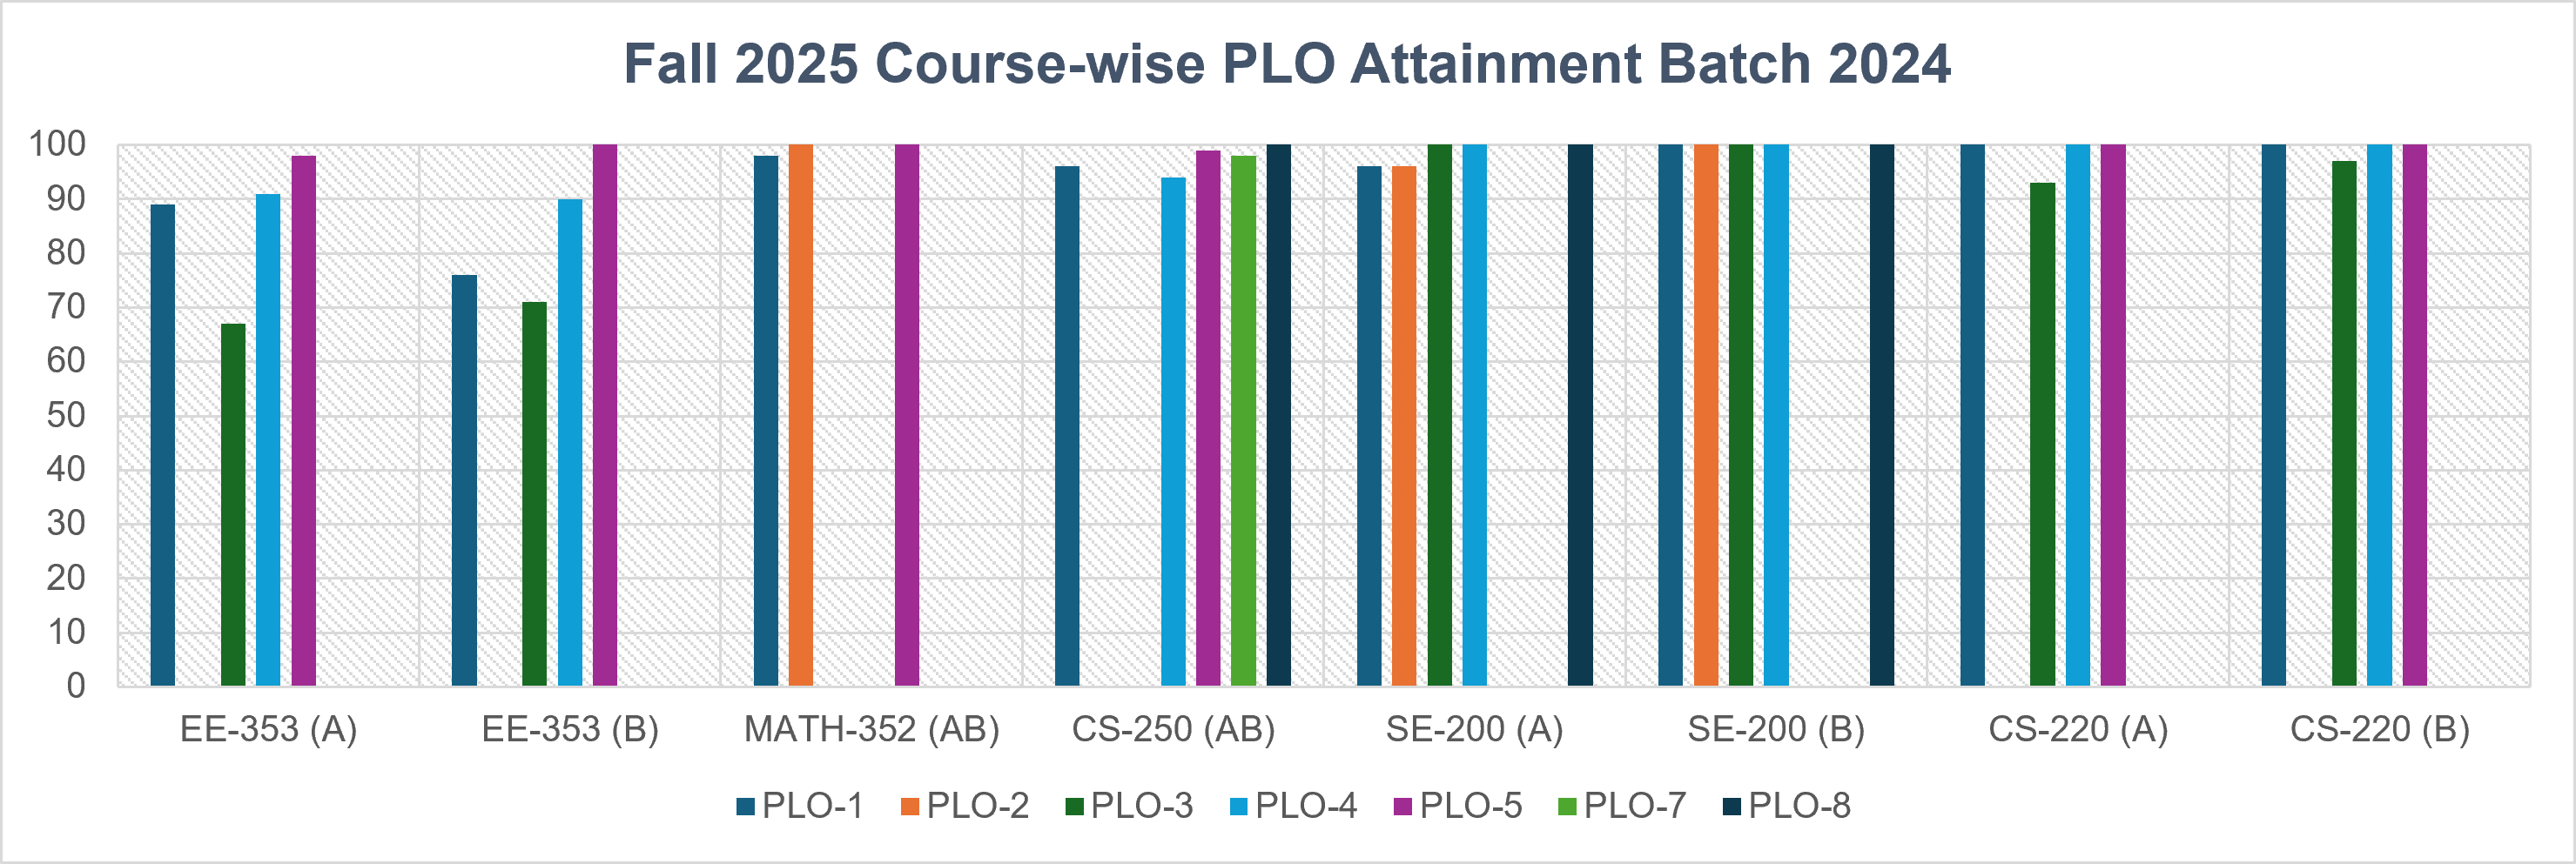
\includegraphics[width=0.95\textwidth]{images/criterion_2/media/image29.png}
\caption{2K24 Batch course-wise PLO attainment for Fall 2025}
\end{figure}

\begin{figure}[H]
\centering
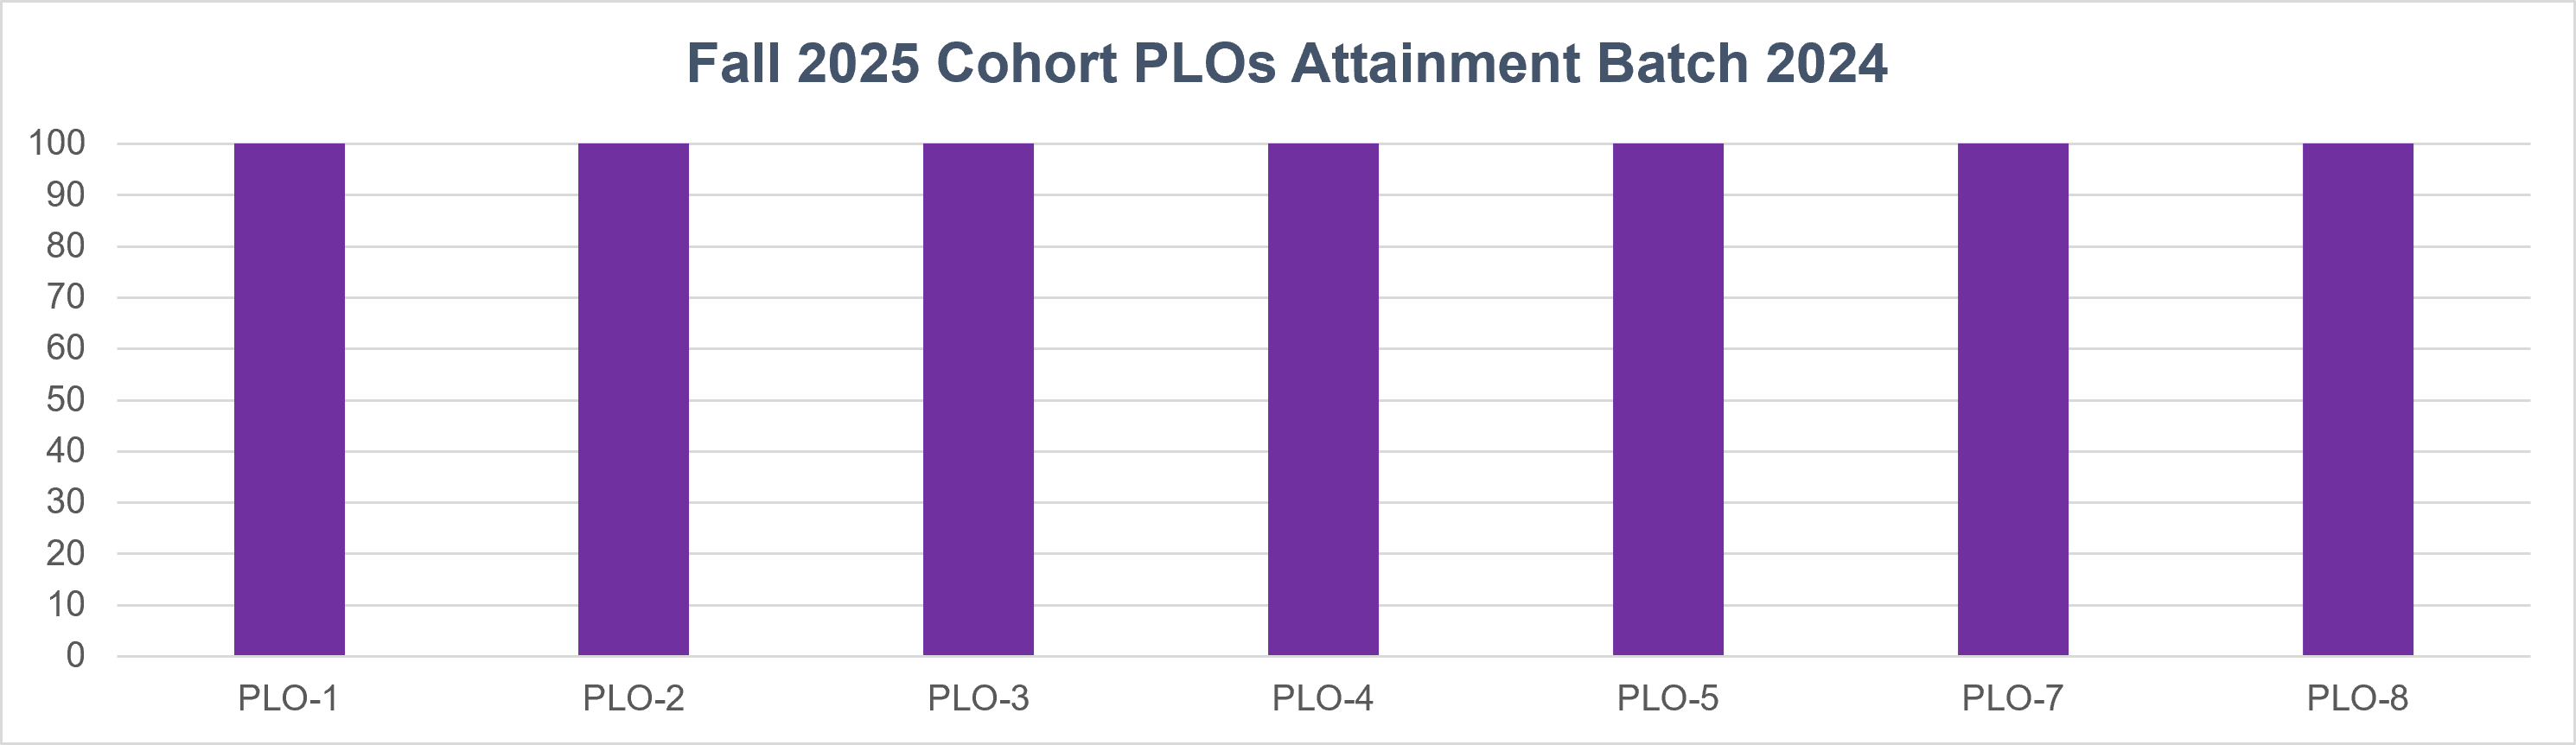
\includegraphics[width=0.95\textwidth]{images/criterion_2/media/image30.png}
\caption{2K24 Batch cohort PLO attainment against the 60\% KPI.}
\label{figure:2024 Batch cohort PLO attainment against}
\end{figure}

\subsection{2K25 Batch Fall 2025 Semester Results}

The results for 2K25 batch are given in Figure~\ref{figure:2025 Batch Result for All Courses} to Figure~\ref{figure:2025 Batch cohort PLO attainment}. It can be seen that the 2K25 batch has attained the assessed CLOs as well as the mapped PLOs on cohort level as per the set KPIs.

\begin{figure}[H]
\centering
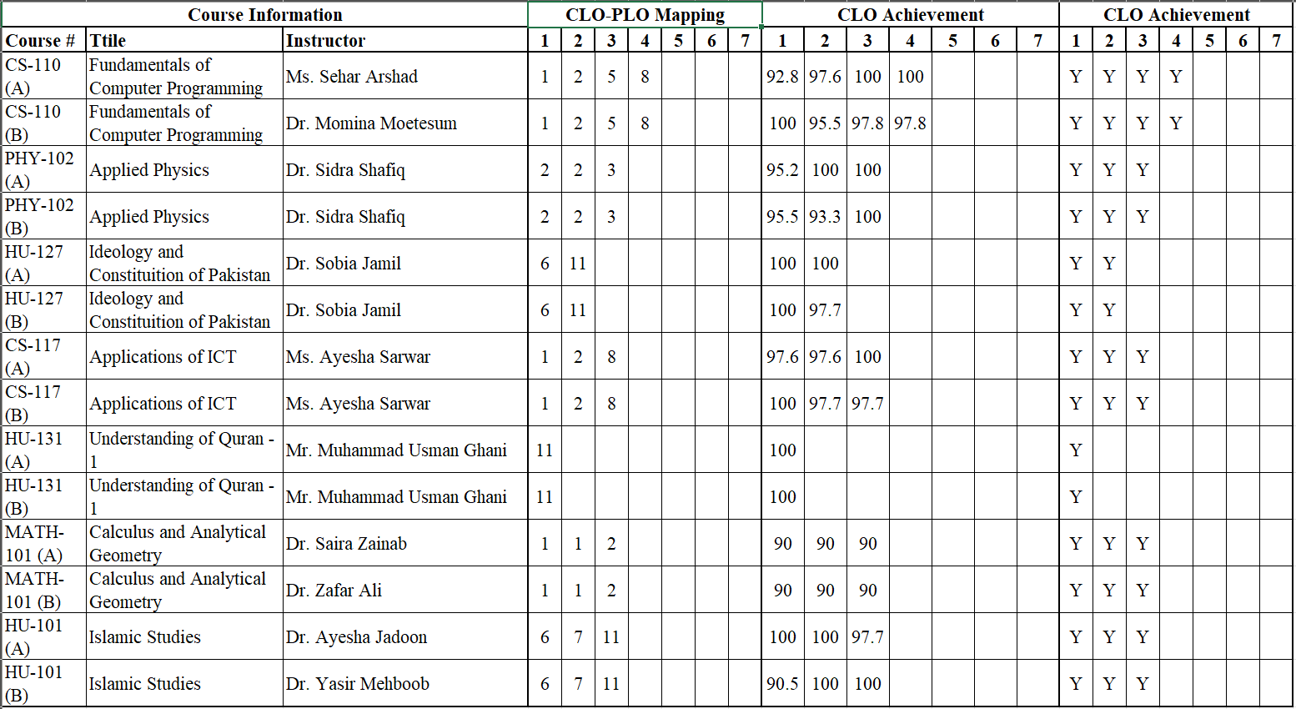
\includegraphics[width=0.98\linewidth]{images/criterion_2/media/image31.png}
\par\medskip
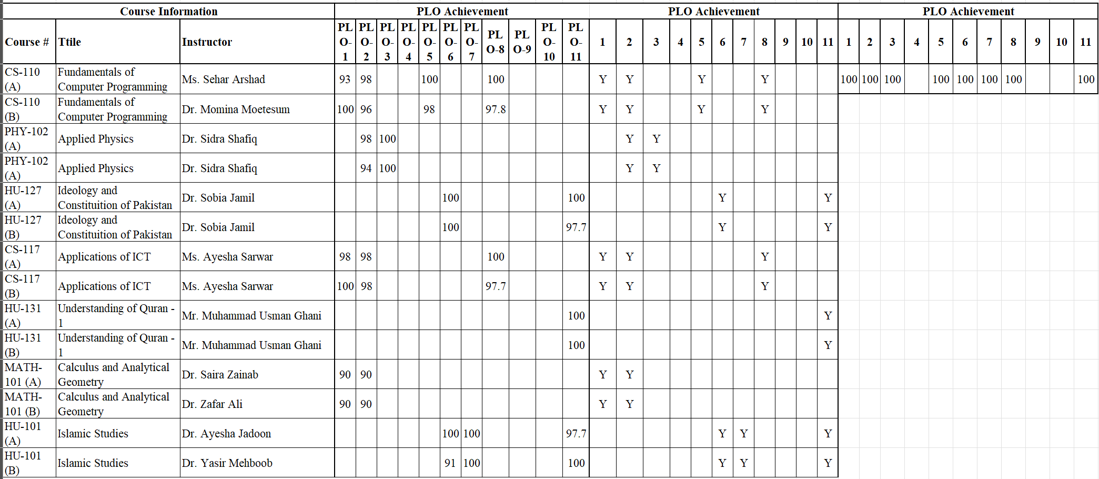
\includegraphics[width=0.98\linewidth]{images/criterion_2/media/image32.png}
\caption{2K25 Batch Result for All Courses in Fall 2025 Semester}
\label{figure:2025 Batch Result for All Courses}
\end{figure}

\begin{figure}[H]
\centering
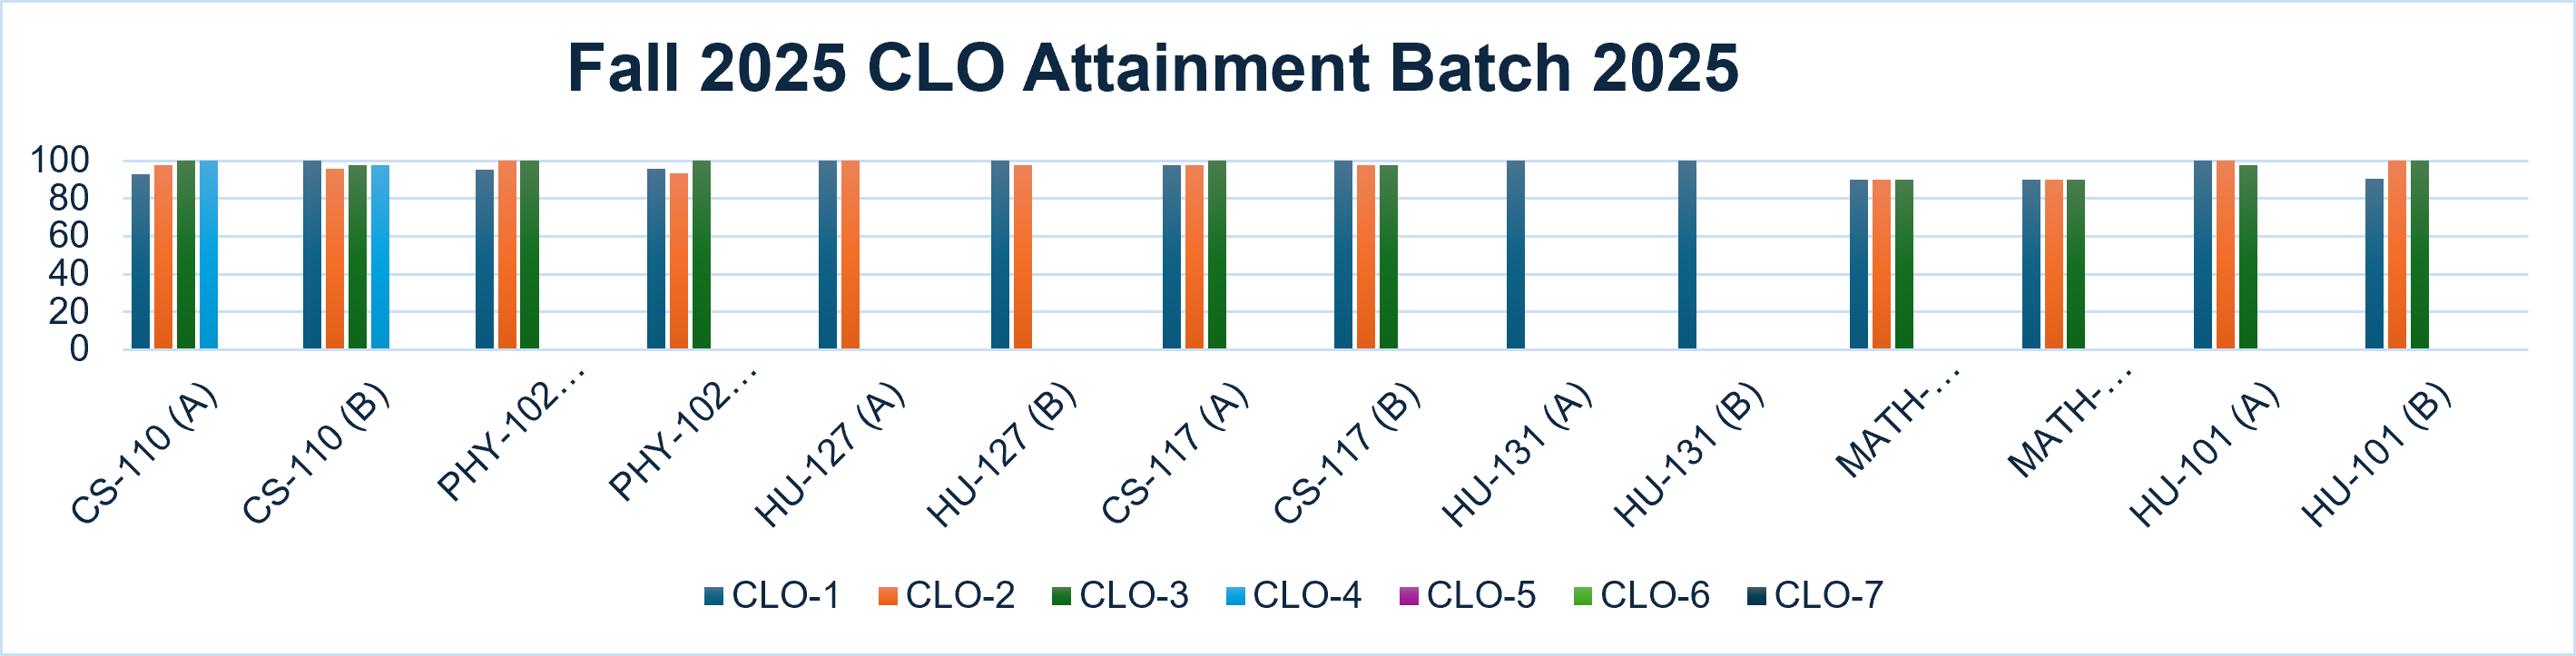
\includegraphics[width=0.95\textwidth]{images/criterion_2/media/image33.png}
\caption{2K25 Batch cohort CLO attainment for all courses in Fall 2025.}
\end{figure}

\begin{figure}[H]
\centering
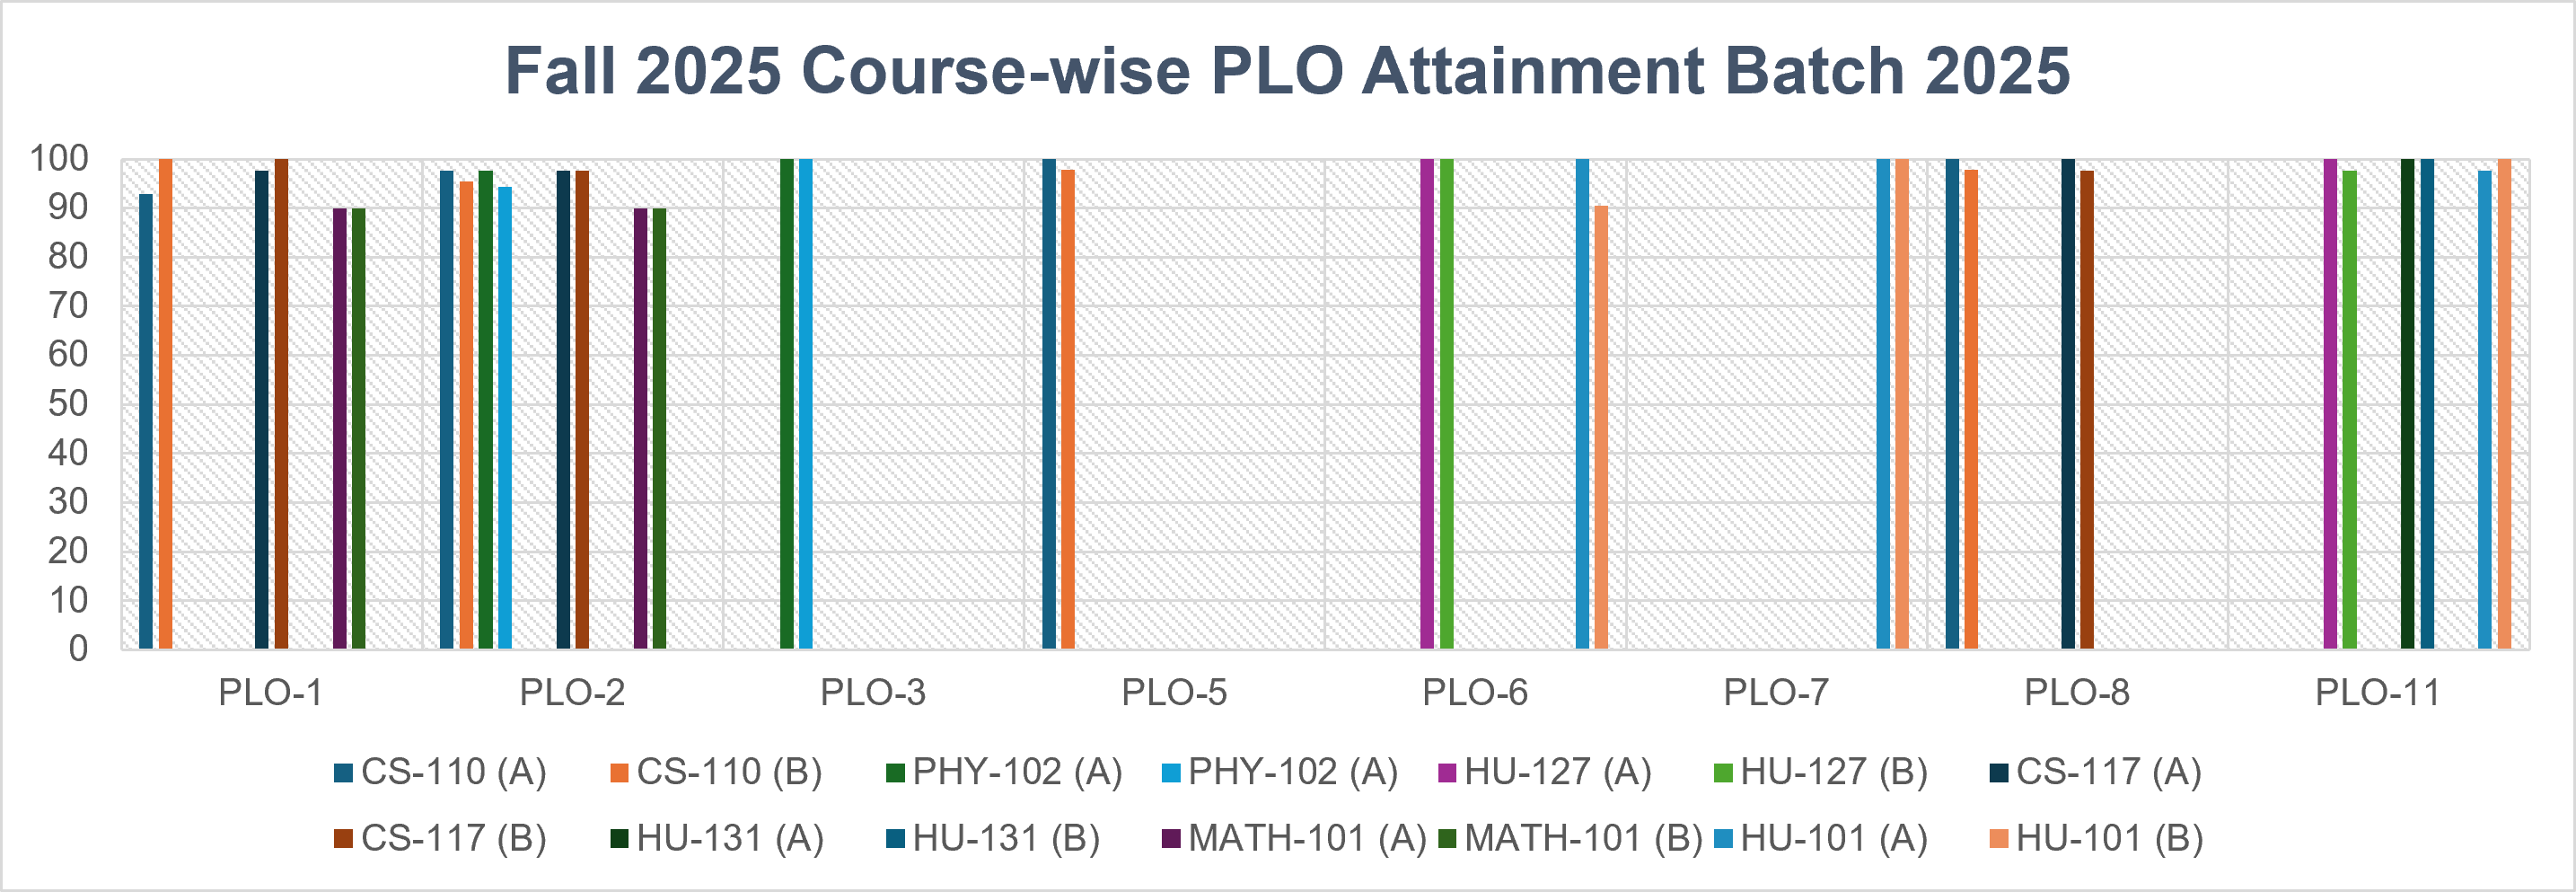
\includegraphics[width=0.95\textwidth]{images/criterion_2/media/image34.png}
\caption{2K25 Batch course-wise PLO attainment for Fall 2025.}
\end{figure}

\begin{figure}[H]
\centering
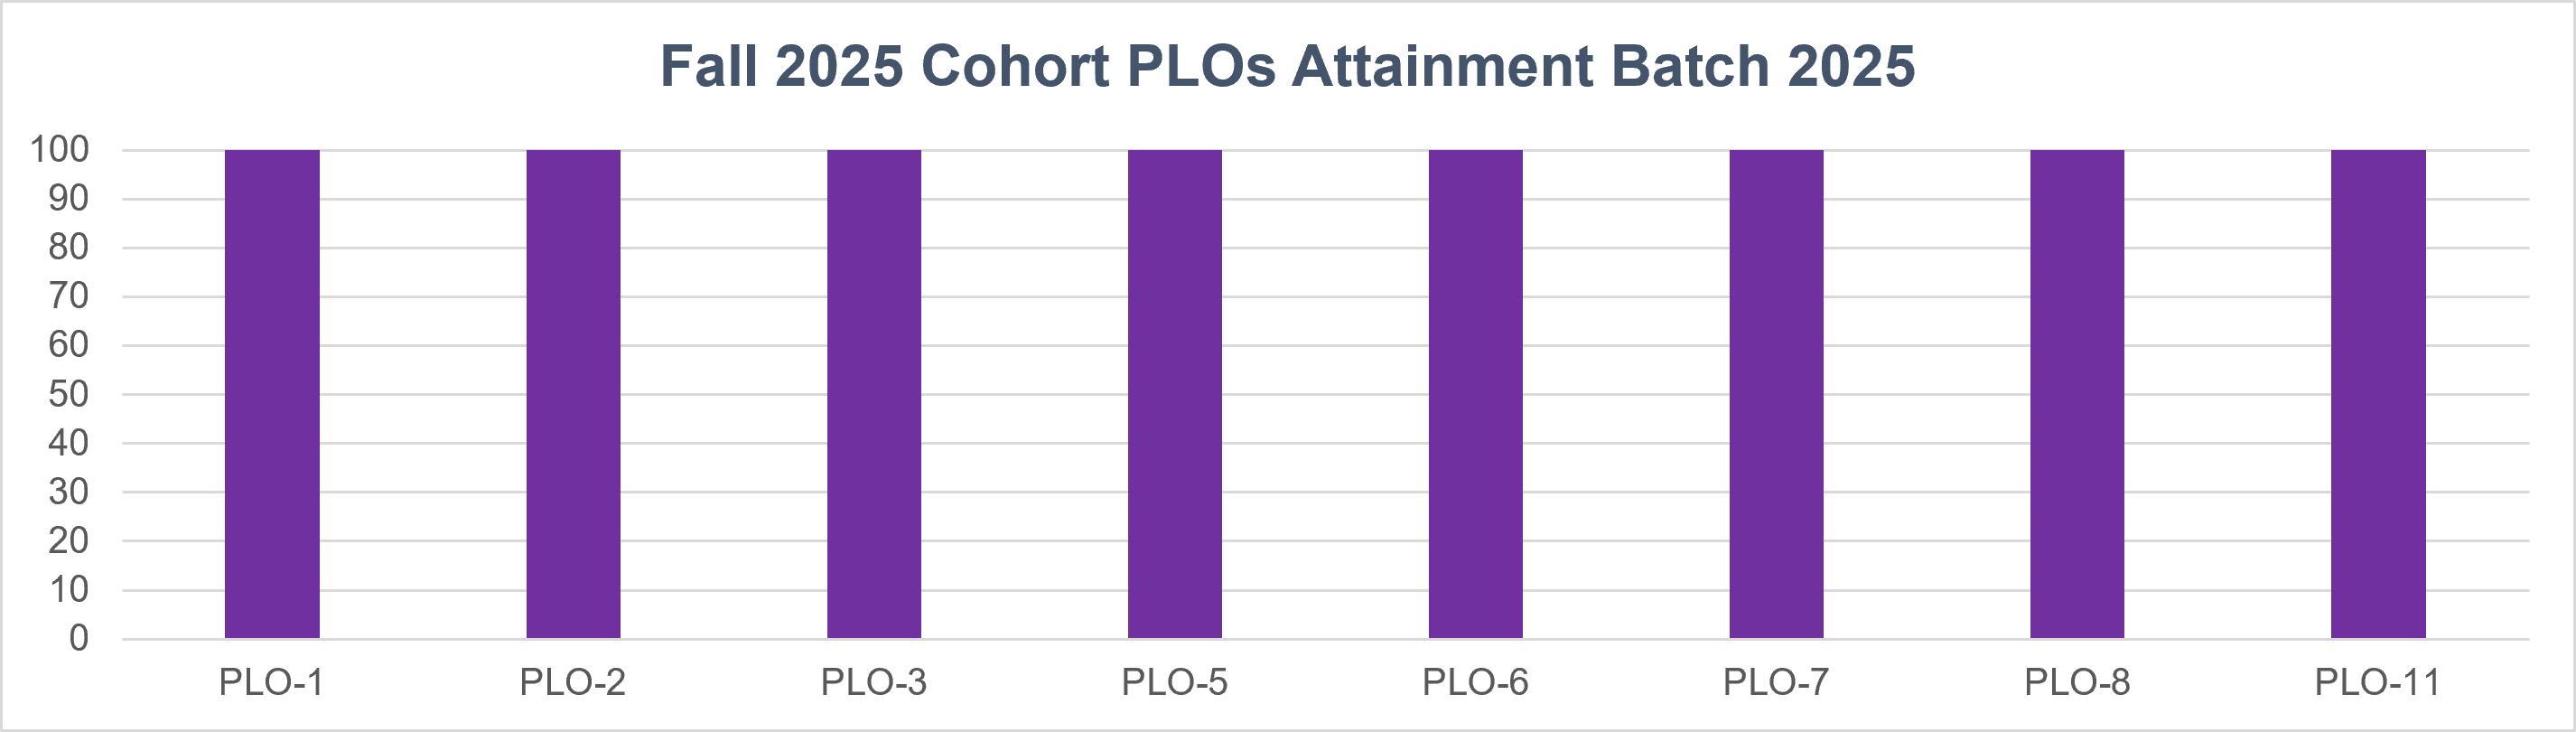
\includegraphics[width=0.95\textwidth]{images/criterion_2/media/image35.png}
\caption{2K25 Batch cohort PLO attainment against the 60\% KPI.}
\label{figure:2025 Batch cohort PLO attainment}
\end{figure}

\section{Internship Feedback Form}
\label{annex:internship-feedback-form}
%\includefullannexure{appendices/criterion_2/Internship Feedback Form.pdf}
\begin{figure}[H]
\centering
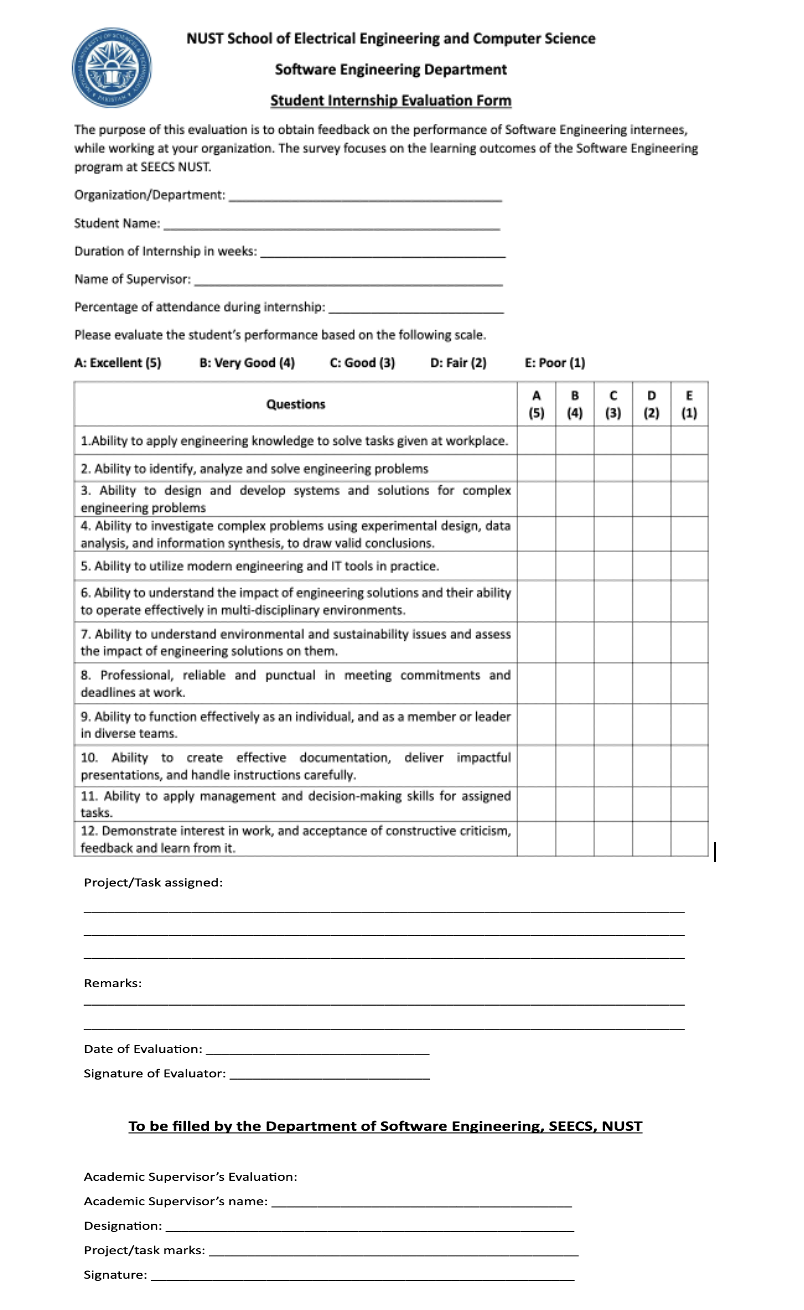
\includegraphics[width=1.0\textwidth]{images/criterion_2/media/internship form.png}
\caption{Internship Feedback Form}
\label{figure:internship form}
\end{figure}

\section{Internship Feedback Analysis}
\label{annex:internship-feedback-analysis}
This analysis evaluates the attainment of Program Learning Outcomes (PLOs) for the Bachelor of Engineering in Software Engineering (BESE) program across three consecutive intake batches: 2K21, 2K22, and 2K23. The assessment is based on industry employer feedback collected via a 5-point Likert scale (where 5 is the highest/excellent and 1 is the lowest/poor) during student internships. The sample sizes for the feedback is given in Figure~\ref{fig:internship-sample-sizes}.

\begin{figure}[H]
\centering
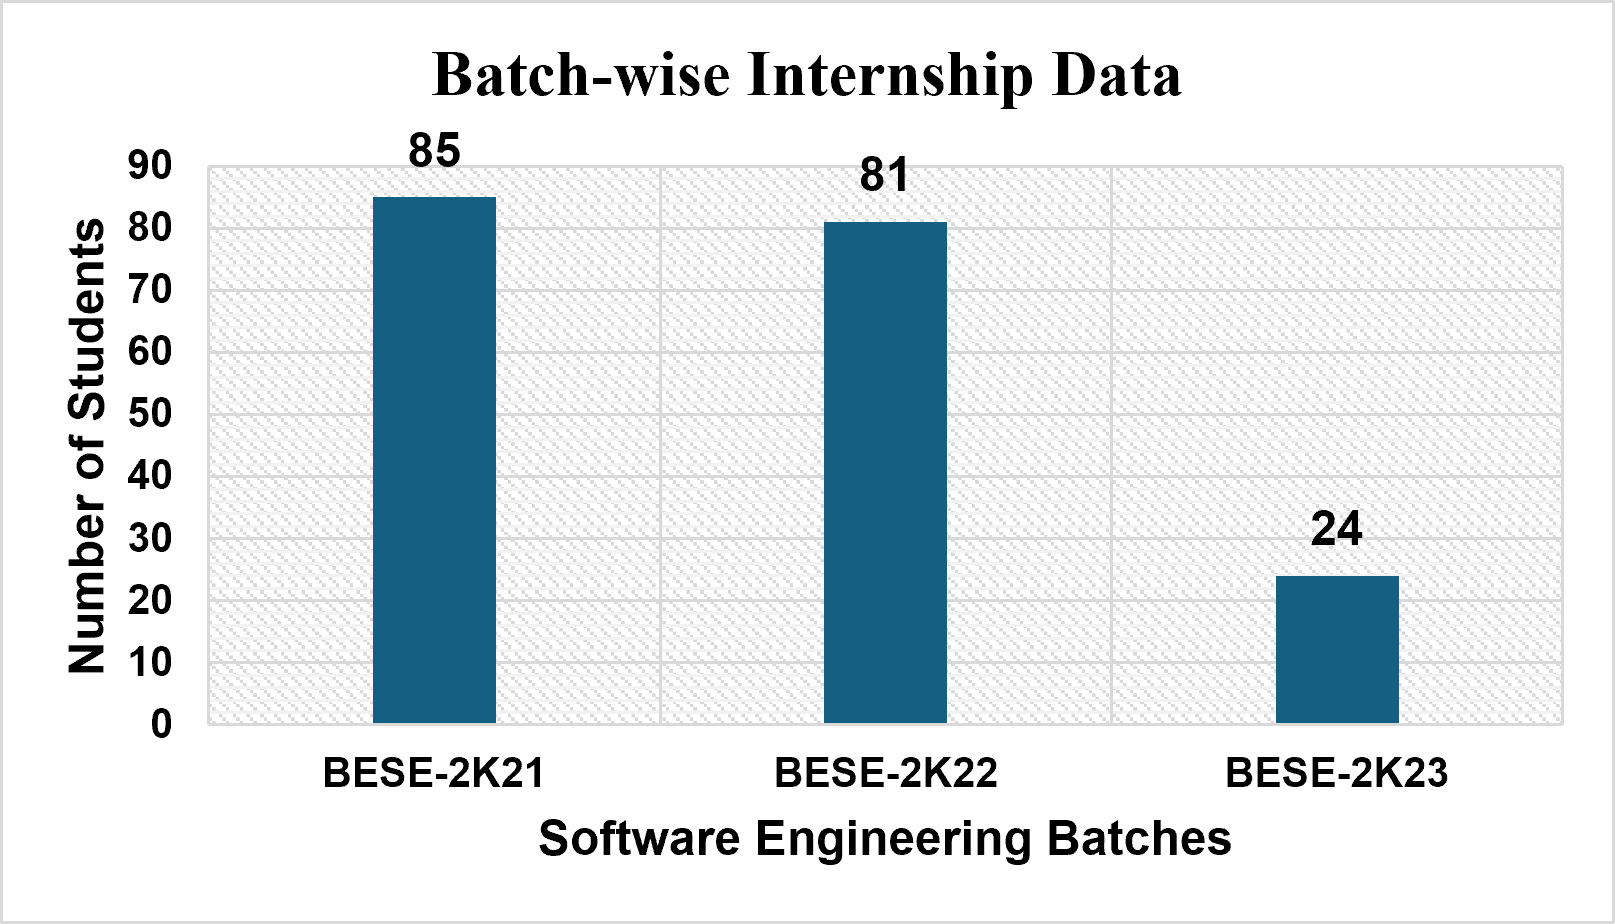
\includegraphics[width=0.78\textwidth]{images/criterion_2/media/image36.png}
\caption{Batch-wise sample sizes for internship employer feedback.}
\label{fig:internship-sample-sizes}
\end{figure}

\subsection{Batch-Wise PLO Attainment Performance}

\textbf{1.\ Batch 2K21 Analysis}

Employers overall rated the 2K21 batch very highly, with negligible negative feedback (scores of 1 or 2) across almost all outcomes. Figure~\ref{figure:PLO attainment based on internship 2K21} shows the average PLO attainment plots for the BESE 2K21 batch. Table~\ref{table:PLO attainment based on internship 2K21} shows the number of employer responses obtained for each rubric.

\begin{itemize}
\item \textbf{Highest Attainment:} \textbf{PLO 11} (Management and decision-making; 46 scores of 5) and \textbf{PLO 12} (Interest in work and handling feedback; 43 scores of 5). This indicates strong soft skills, adaptability, and professional maturity.
\item \textbf{Areas for Growth:} \textbf{PLO 3} (Design and development; 29 scores of 5) and \textbf{PLO 4} (Investigation of complex problems; 30 scores of 5) received slightly lower top-tier scores, showing that while students are competent, complex problem-solving and deep engineering design require further reinforcement.
\end{itemize}

\begin{figure}[H]
\centering
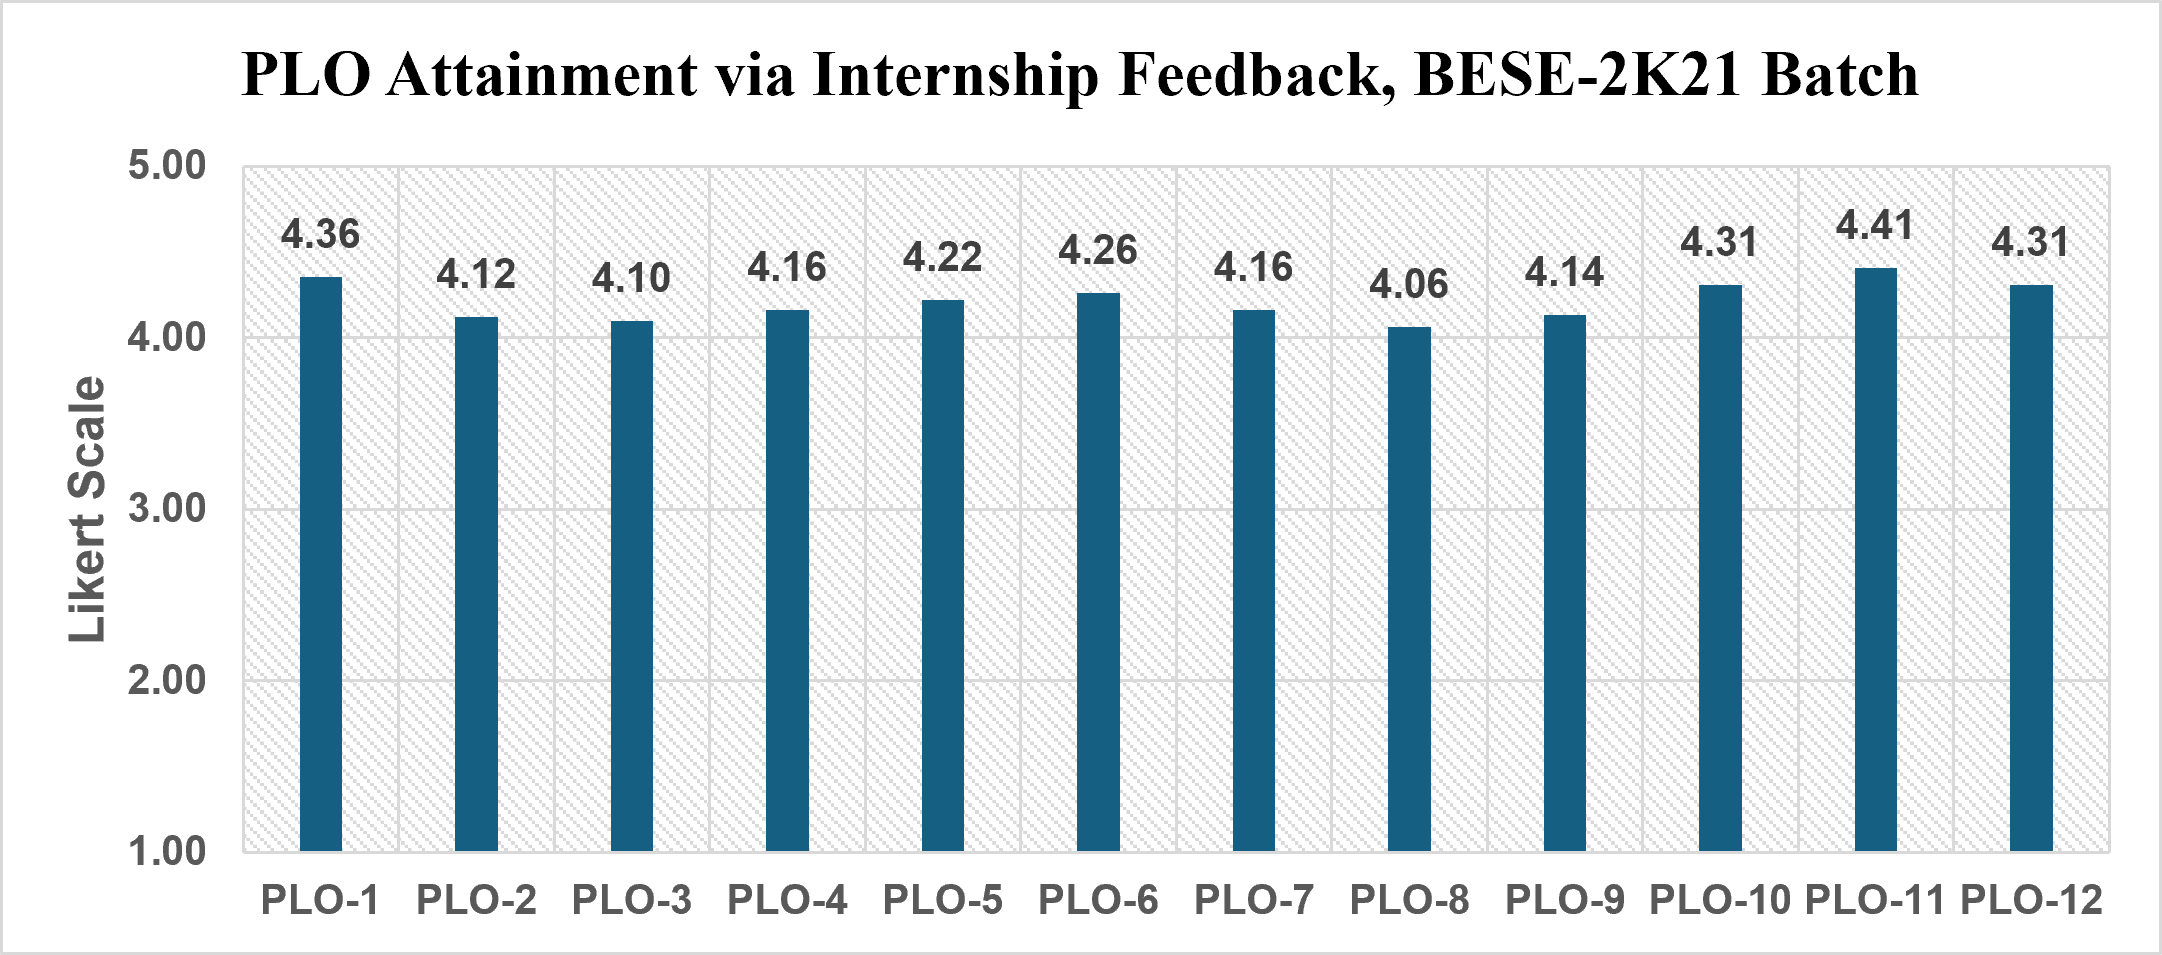
\includegraphics[width=0.90\textwidth]{images/criterion_2/media/image37.png}
\caption{PLO attainment based on internship feedback for the BESE 2K21 Batch.}
\label{figure:PLO attainment based on internship 2K21}
\end{figure}

\begin{table}[H]
\centering
\caption{Internship Feedback for the Batch 2K21}
\begin{tabular}{>{\centering\arraybackslash}p{0.06\textwidth}
                >{\raggedright\arraybackslash}p{0.5\textwidth}
                >{\centering\arraybackslash}p{0.05\textwidth}
                >{\centering\arraybackslash}p{0.05\textwidth}
                >{\centering\arraybackslash}p{0.05\textwidth}
                >{\centering\arraybackslash}p{0.05\textwidth}
                >{\centering\arraybackslash}p{0.05\textwidth}}
\toprule
\textbf{PLO} & \textbf{Rubric} & \textbf{5} & \textbf{4} & \textbf{3} & \textbf{2} & \textbf{1} \\
\midrule
1  & Ability to apply engineering knowledge to solve tasks given at workplace. & 39 & 32 & 10 & 0 & 0 \\
2  & Ability to identify, analyze and solve engineering problems & 31 & 32 & 15 & 3 & 0 \\
3  & Ability to design and develop systems and solutions for complex engineering problems & 29 & 33 & 17 & 2 & 0 \\
4  & Ability to investigate complex problems using experimental design, data analysis, and information synthesis, to draw valid conclusions. & 30 & 35 & 15 & 1 & 0 \\
5  & Ability to utilize modern engineering and IT tools in practice. & 41 & 22 & 13 & 5 & 0 \\
6  & Ability to understand the impact of engineering solutions and their ability to operate effectively in multi-disciplinary environments. & 32 & 38 & 11 & 0 & 0 \\
7  & Ability to understand environmental and sustainability issues and assess the impact of engineering solutions on them & 34 & 27 & 19 & 1 & 0 \\
8  & Professional, reliable and punctual in meeting commitments and deadlines at work. & 31 & 27 & 20 & 3 & 0 \\
9  & Ability to function effectively as an individual, and as a member or leader in diverse teams. & 35 & 27 & 14 & 5 & 0 \\
10 & Ability to create effective documentation, deliver impactful presentations, and handle instructions carefully & 37 & 32 & 12 & 0 & 0 \\
11 & Ability to apply management and decision-making skills for assigned tasks & 46 & 23 & 11 & 1 & 0 \\
12 & Demonstrate interest in work, and acceptance of constructive criticism, feedback and learn from it. & 43 & 24 & 10 & 4 & 0 \\
\bottomrule
\end{tabular}
\label{table:PLO attainment based on internship 2K21}
\end{table}

\textbf{2.\ Batch 2K22 Analysis}

Batch 2K22 sustained high levels of satisfaction, showing slight shifts in technical versus behavioral performance. Figure~\ref{figure:PLO attainment based on internship 2K22} shows the average PLO attainment plots for the BESE 2K22 batch. Table~\ref{table:PLO attainment based on internship 2K22} shows the number of employer responses obtained for each rubric.

\begin{itemize}
\item \textbf{Highest Attainment:} \textbf{PLO 12} (Interest in work and feedback; 49 scores of 5) and \textbf{PLO 1} (Applying engineering knowledge; 47 scores of 5). Employers found these students highly motivated and technically grounded right at the workplace entry level.
\item \textbf{Areas for Growth:} \textbf{PLO 8} (Professionalism, reliability, and punctuality) scored the lowest in the top tier (only 26 scores of 5), though it was heavily compensated by 39 scores of 4. \textbf{PLO 2} (Problem identification and analysis) also showed a higher volume of moderate ratings (20 scores of 3).
\end{itemize}

\begin{figure}[H]
\centering
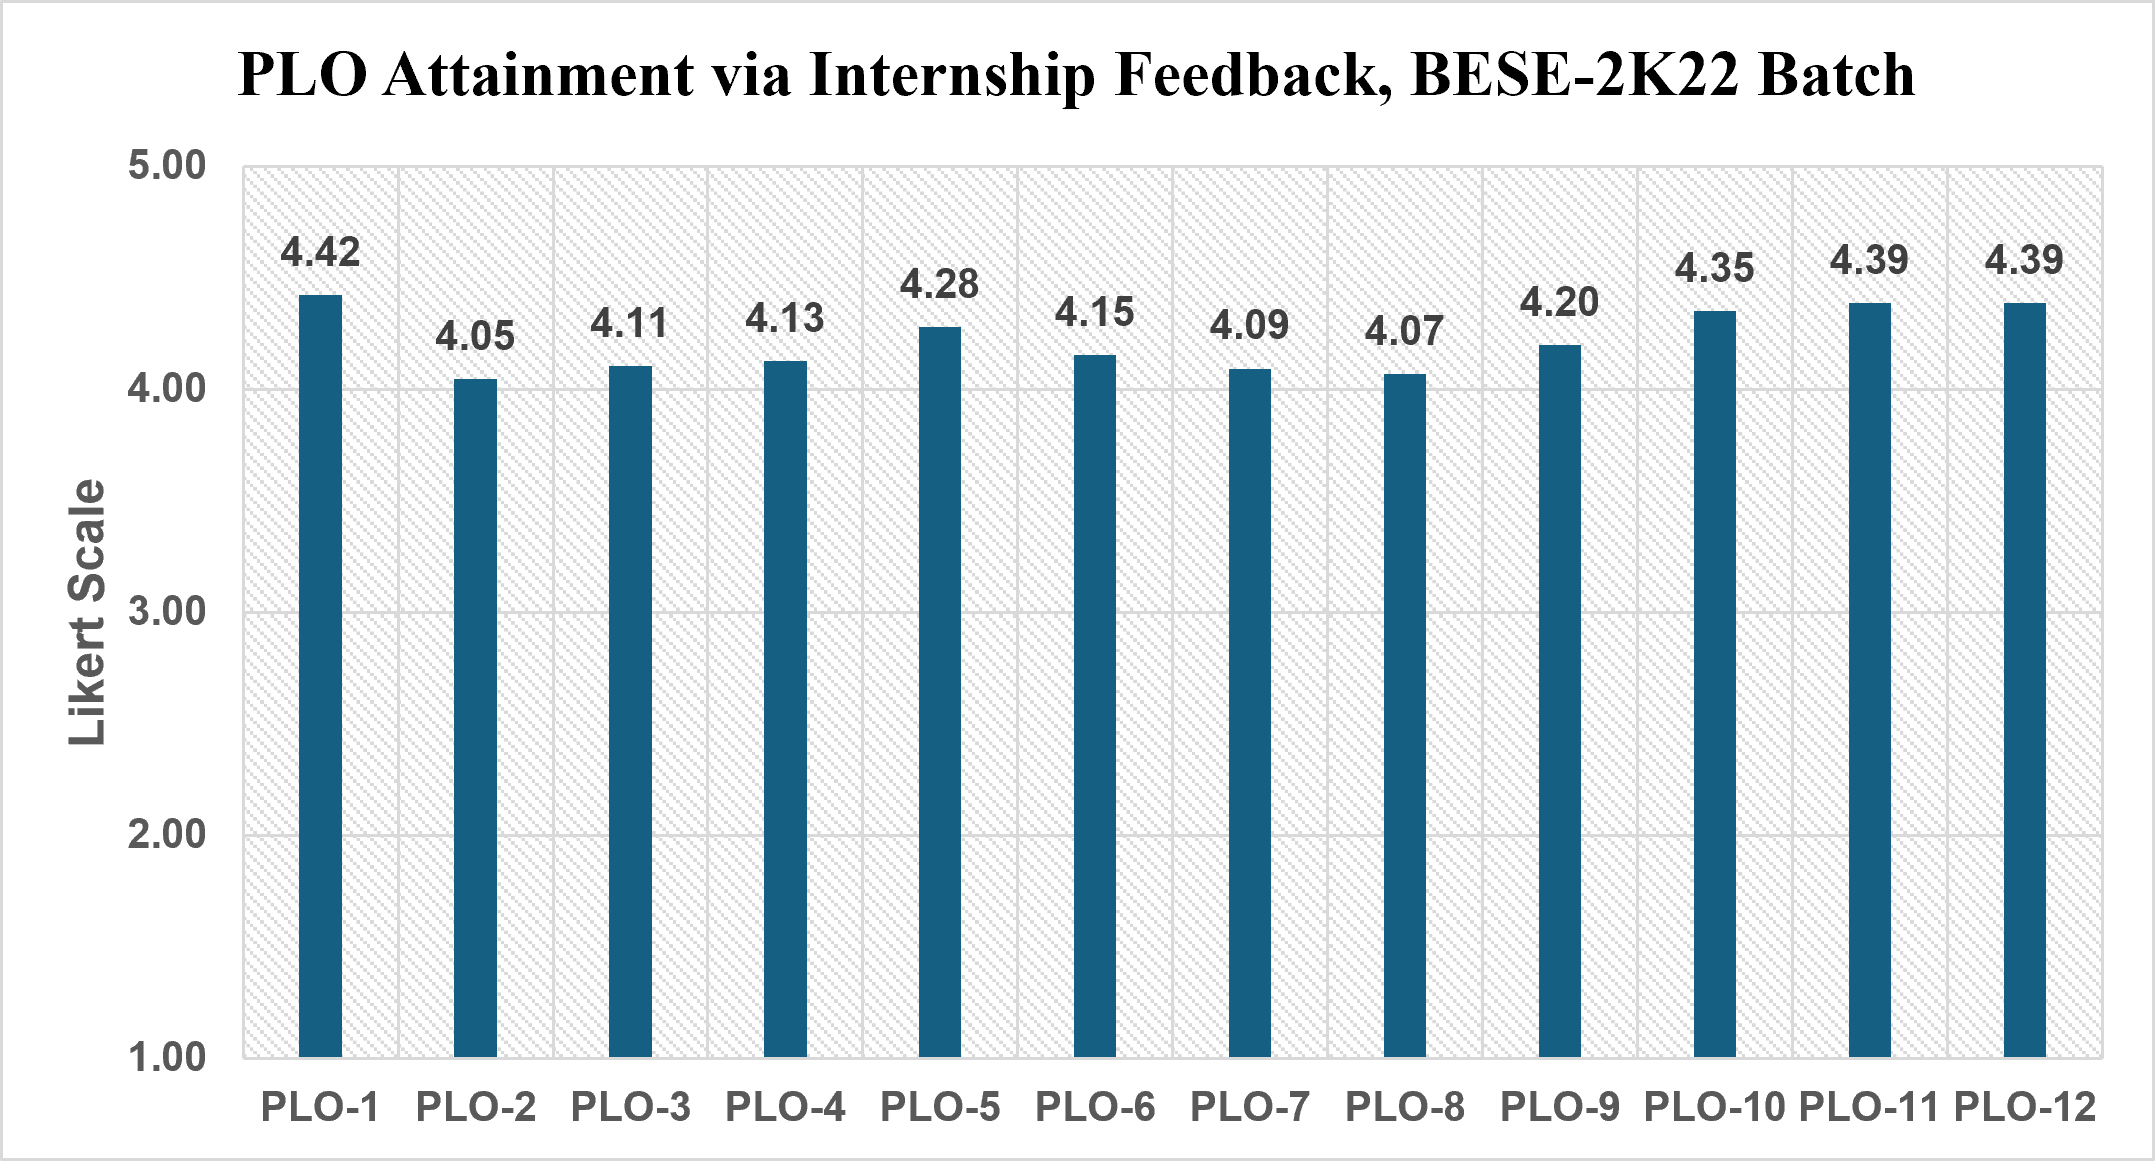
\includegraphics[width=0.90\textwidth]{images/criterion_2/media/image38.png}
\caption{PLO attainment based on internship feedback for the BESE 2K22 Batch.}
\label{figure:PLO attainment based on internship 2K22}
\end{figure}

\begin{longtable}{>{\centering\arraybackslash}p{0.06\textwidth}
                  >{\raggedright\arraybackslash}p{0.5\textwidth}
                  >{\centering\arraybackslash}p{0.05\textwidth}
                  >{\centering\arraybackslash}p{0.05\textwidth}
                  >{\centering\arraybackslash}p{0.05\textwidth}
                  >{\centering\arraybackslash}p{0.05\textwidth}
                  >{\centering\arraybackslash}p{0.05\textwidth}}

\caption{Internship Feedback for the Batch 2K22}
\label{table:PLO attainment based on internship 2K22} \\

\toprule
\textbf{PLO} & \textbf{Rubric} & \textbf{5} & \textbf{4} &
\textbf{3} & \textbf{2} & \textbf{1} \\
\midrule
\endfirsthead

\multicolumn{7}{c}%
{\tablename\ \thetable{} -- continued from previous page} \\
\toprule
\textbf{PLO} & \textbf{Rubric} & \textbf{5} & \textbf{4} &
\textbf{3} & \textbf{2} & \textbf{1} \\
\midrule
\endhead

\midrule
\multicolumn{7}{r}{Continued on next page} \\
\endfoot

\bottomrule
\endlastfoot

1  & Ability to apply engineering knowledge to solve tasks given at workplace. & 47 & 27 & 11 & 0 & 0 \\
2  & Ability to identify, analyze and solve engineering problems & 28 & 35 & 20 & 2 & 0 \\
3  & Ability to design and develop systems and solutions for complex engineering problems & 33 & 29 & 22 & 1 & 0 \\
4  & Ability to investigate complex problems using experimental design, data analysis, and information synthesis, to draw valid conclusions. & 29 & 40 & 14 & 2 & 0 \\
5  & Ability to utilize modern engineering and IT tools in practice. & 40 & 33 & 8 & 4 & 0 \\
6  & Ability to understand the impact of engineering solutions and their ability to operate effectively in multi-disciplinary environments. & 31 & 38 & 14 & 2 & 0 \\
7  & Ability to understand environmental and sustainability issues and assess the impact of engineering solutions on them & 32 & 30 & 22 & 1 & 0 \\
8  & Professional, reliable and punctual in meeting commitments and deadlines at work. & 26 & 39 & 20 & 0 & 0 \\
9  & Ability to function effectively as an individual, and as a member or leader in diverse teams. & 36 & 31 & 17 & 1 & 0 \\
10 & Ability to create effective documentation, deliver impactful presentations, and handle instructions carefully & 45 & 25 & 15 & 0 & 0 \\
11 & Ability to apply management and decision-making skills for assigned tasks & 46 & 27 & 11 & 1 & 0 \\
12 & Demonstrate interest in work, and acceptance of constructive criticism, feedback and learn from it. & 49 & 23 & 11 & 1 & 1 \\

\end{longtable}

\textbf{3.\ Batch 2K23 Analysis}

While the data pool for 2K23 is smaller (interim data), the trend remains consistently positive, skewed heavily toward scores of 4 and 5. Figure~\ref{figure:PLO attainment based on internship 2K23} shows the average PLO attainment plots for the BESE 2K23 batch. Table~\ref{table:PLO attainment based on internship 2K23} shows the number of employer responses obtained for each rubric.

\begin{itemize}
\item \textbf{Highest Attainment:} \textbf{PLO 1} (Applying engineering knowledge), \textbf{PLO 11} (Management/decision-making), and \textbf{PLO 12} (Interest in work/feedback) all tied with 19 scores of 5 out of 24.
\item \textbf{Areas for Growth:} \textbf{PLO 7} (Environmental and sustainability issues) was noticeably weaker in top-tier performance, receiving only 8 scores of 5, though it was balanced by 14 scores of 4.
\end{itemize}

\begin{figure}[H]
\centering
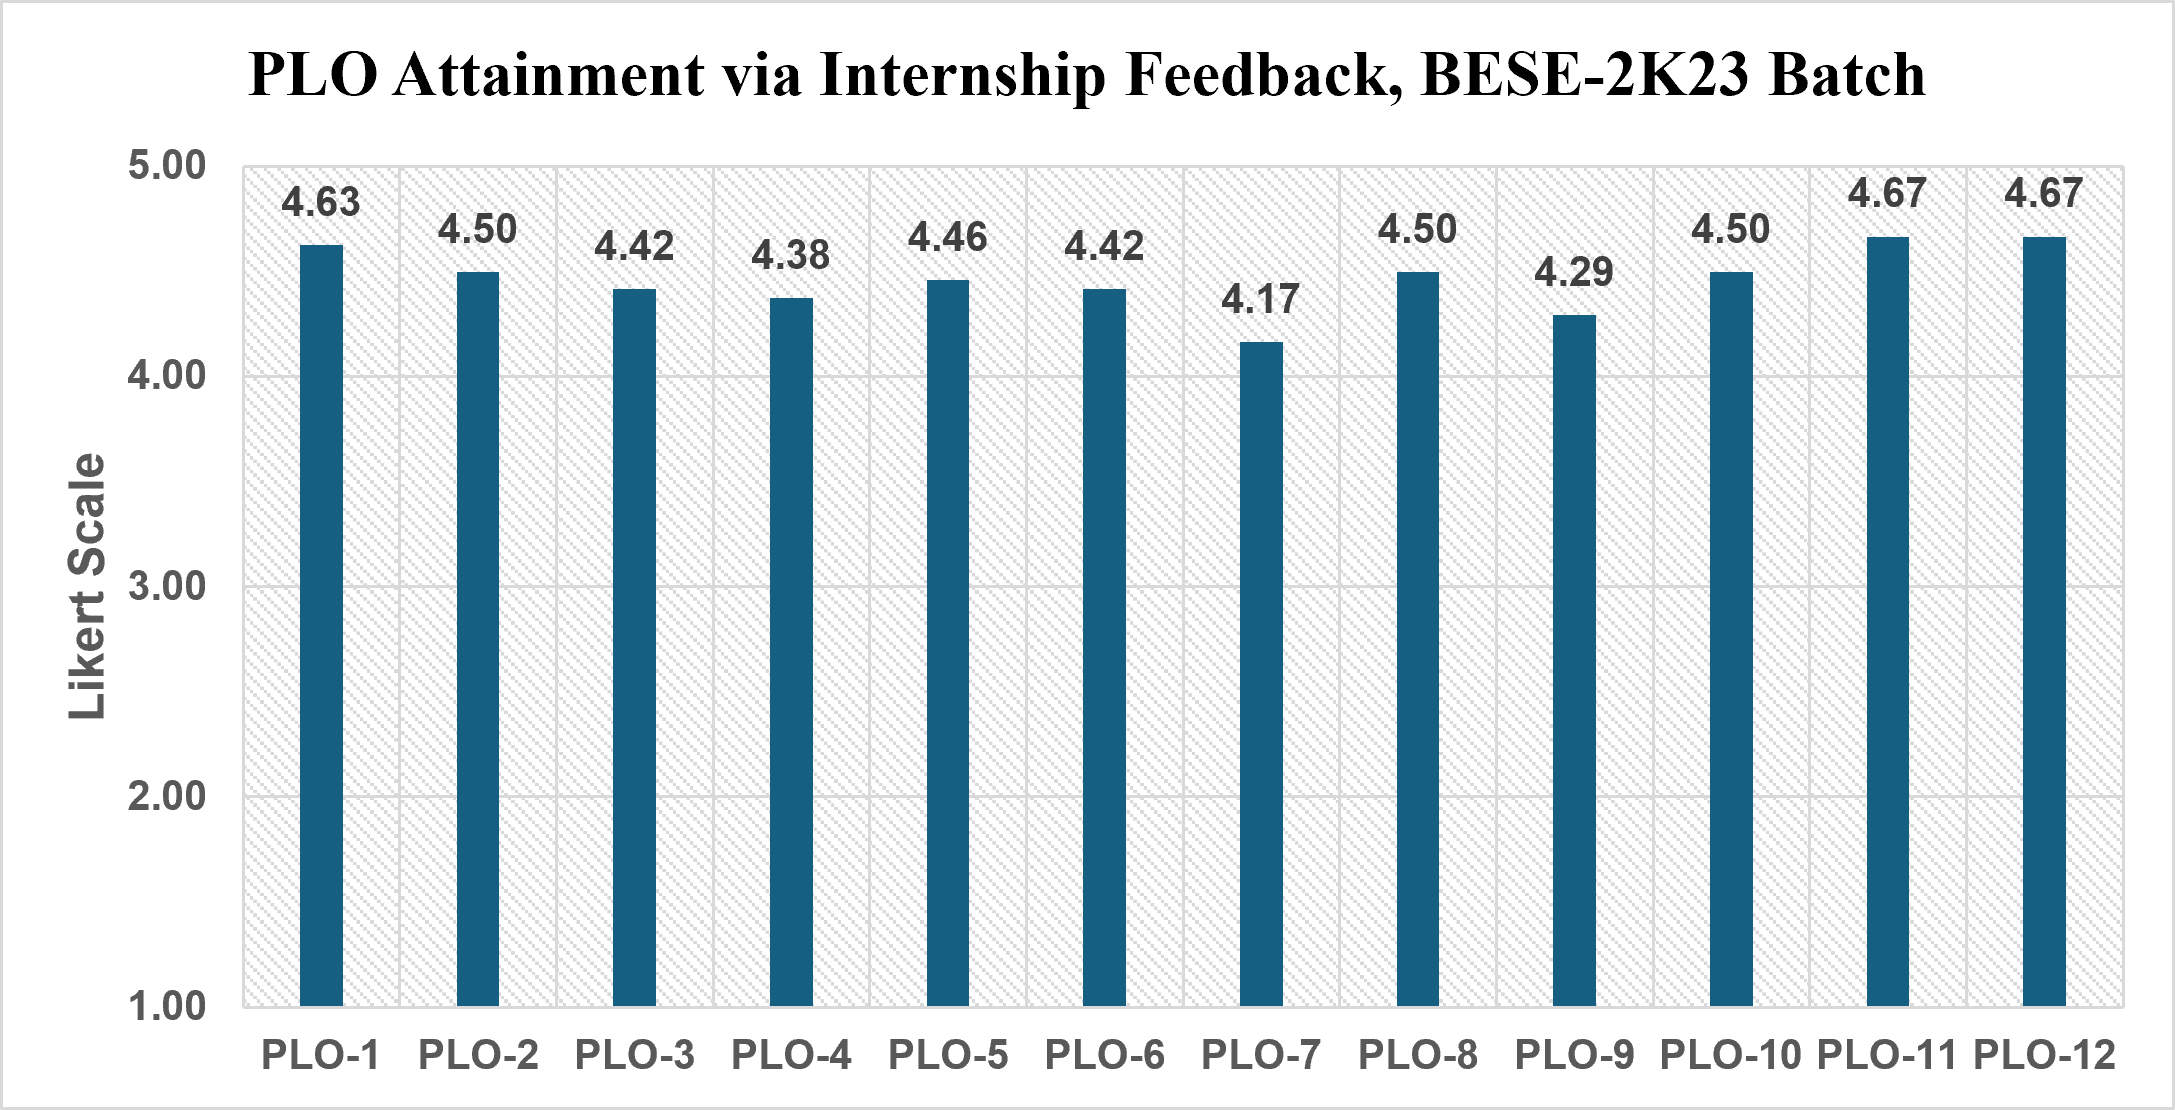
\includegraphics[width=0.90\textwidth]{images/criterion_2/media/image39.png}
\caption{PLO attainment based on internship feedback for the BESE 2K23 Batch.}
\label{figure:PLO attainment based on internship 2K23}
\end{figure}

\begin{table}[H]
\centering
\caption{Internship Feedback for the Batch 2K23}
\begin{tabular}{>{\centering\arraybackslash}p{0.06\textwidth}
                >{\raggedright\arraybackslash}p{0.5\textwidth}
                >{\centering\arraybackslash}p{0.05\textwidth}
                >{\centering\arraybackslash}p{0.05\textwidth}
                >{\centering\arraybackslash}p{0.05\textwidth}
                >{\centering\arraybackslash}p{0.05\textwidth}
                >{\centering\arraybackslash}p{0.05\textwidth}}
\toprule
\textbf{PLO} & \textbf{Rubric} & \textbf{5} & \textbf{4} & \textbf{3} & \textbf{2} & \textbf{1} \\
\midrule
1  & Ability to apply engineering knowledge to solve tasks given at workplace. & 19 & 3 & 1 & 0 & 1 \\
2  & Ability to identify, analyze and solve engineering problems & 16 & 6 & 1 & 0 & 1 \\
3  & Ability to design and develop systems and solutions for complex engineering problems & 14 & 8 & 1 & 0 & 1 \\
4  & Ability to investigate complex problems using experimental design, data analysis, and information synthesis, to draw valid conclusions. & 13 & 9 & 1 & 0 & 1 \\
5  & Ability to utilize modern engineering and IT tools in practice. & 15 & 7 & 1 & 0 & 1 \\
6  & Ability to understand the impact of engineering solutions and their ability to operate effectively in multi-disciplinary environments. & 15 & 6 & 2 & 0 & 1 \\
7  & Ability to understand environmental and sustainability issues and assess the impact of engineering solutions on them & 8 & 14 & 1 & 0 & 1 \\
8  & Professional, reliable and punctual in meeting commitments and deadlines at work. & 16 & 6 & 1 & 0 & 1 \\
9  & Ability to function effectively as an individual, and as a member or leader in diverse teams. & 14 & 5 & 4 & 0 & 1 \\
10 & Ability to create effective documentation, deliver impactful presentations, and handle instructions carefully & 16 & 6 & 1 & 0 & 1 \\
11 & Ability to apply management and decision-making skills for assigned tasks & 19 & 4 & 0 & 0 & 1 \\
12 & Demonstrate interest in work, and acceptance of constructive criticism, feedback and learn from it. & 19 & 4 & 0 & 0 & 1 \\
\bottomrule
\end{tabular}
\label{table:PLO attainment based on internship 2K23}
\end{table}

\textbf{Comparative PLO Performance Matrix}

To easily spot macro trends, the Table~\ref{table: Comparative PLO Performance Matrix} highlights the percentage of Excellent to Very Good ratings (Scores 4 \& 5 combined) for each PLO across the three cohorts:

\begin{table}[H]
\footnotesize
\centering
\caption{Comparative PLO Performance Matrix -- Internship Feedback (Scores 4 \& 5 Combined)}
\label{table: Comparative PLO Performance Matrix}
\begin{tabular}{>{\centering\arraybackslash}p{0.09\textwidth}
                >{\raggedright\arraybackslash}p{0.36\textwidth}
                >{\centering\arraybackslash}p{0.15\textwidth}
                >{\centering\arraybackslash}p{0.15\textwidth}
                >{\centering\arraybackslash}p{0.15\textwidth}}
\toprule
\textbf{PLOs} & \textbf{Rubric Summary} & \textbf{Batch 2K21} & \textbf{Batch 2K22} & \textbf{Batch 2K23} \\
\midrule
PLO 1  & Engineering Knowledge         & 87.7\% & 87.1\% & 91.7\% \\
PLO 2  & Problem Analysis        & 77.8\% & 74.1\% & 91.7\% \\
PLO 3  & Design \& Development of Solutions             & 76.5\% & 72.9\% & 91.7\% \\
PLO 4  & Investigation         & 80.2\% & 81.2\% & 91.7\% \\
PLO 5  & Modern Tool Usage (IT/Engineering)        & 77.8\% & 85.9\% & 91.7\% \\
PLO 6  & The Engineer \& Society & 86.4\% & 81.2\% & 87.5\% \\
PLO 7  & Environment \& Sustainability             & 75.3\% & 72.9\% & 91.7\% \\
PLO 8  & Ethics                                    & 71.6\% & 76.5\% & 91.7\% \\
PLO 9  & Individual \& Team Work                   & 76.5\% & 78.8\% & 79.2\% \\
PLO 10 & Communication Skills            & 85.2\% & 82.4\% & 91.7\% \\
PLO 11 & Project Management                        & 85.2\% & 85.9\% & 95.8\% \\
PLO 12 & Lifelong Learning                         & 82.7\% & 84.7\% & 95.8\% \\
\bottomrule
\end{tabular}
\end{table}

\textbf{Key Observations}

\begin{itemize}
\item \textbf{Consistently Strong Core Competencies:} Across all three batches, \textbf{PLO 1} (Engineering Knowledge), \textbf{PLO 11} (Management/Decision-making), and \textbf{PLO 12} (Lifelong learning/Attitude) are the highest performing areas. Employers consistently note that BESE students have an excellent work ethic, are receptive to constructive criticism, and grasp foundational engineering concepts quickly.
\item \textbf{The ``Complex Engineering'' Bottleneck:} In both 2K21 and 2K22, \textbf{PLO 2} (Problem Analysis) and \textbf{PLO 3} (Design/Development of Solutions) experience a noticeable dip in ``5'' scores, moving into ``4'' and ``3'' ranges. This indicates that while students are capable, executing complex architecture designs or deep systemic troubleshooting in a live corporate environment remains their steepest learning curve.
\item \textbf{Modern Tool Progress:} There is a positive trajectory in \textbf{PLO 5} (Modern Tool Usage), rising from 77.8\% (2K21) to 85.9\% (2K22) in top-tier positive reviews. This suggests that academic curriculum adjustments or lab tools are aligning better with current industry stacks.
\item \textbf{Professionalism \& Teamwork Stabilization:} \textbf{PLO 8} (Punctuality/Commitment) and \textbf{PLO 9} (Teamwork) score slightly lower on absolute ``Excellent'' marks but hold a strong ``Good/Satisfactory'' baseline. This is normal for interns transitioning from a flexible academic environment to rigid corporate schedules.
\end{itemize}

\section{Graduate Exit Survey Form}
\label{annex:graduate-exit-survey-form}
\includefullannexure{appendices/criterion_2/Graduate Exit Form.pdf}


\clearpage
\section{Graduate Exit Survey Analysis}
\label{annex:graduate-exit-survey-analysis}

This annexure evaluates the Program Learning Outcomes (PLOs) attainment for the BESE program based on the Graduate Exit Survey. The survey captures the graduating students' self-assessment of their engineering knowledge, technical skills, and professional attributes on a 5-point Likert scale.

\subsection{Batch 2K20 Analysis}

The graduating batch of 2K20 established a highly stable and balanced baseline across all engineering criteria, with all mean scores residing within a tight, healthy band of \textbf{3.91 to 4.15} as shown in Figure~\ref{fig:exit-survey-2k20} and Table~\ref{table:PLO attainment based on the Graduate Exit}.

\begin{itemize}
\item \textbf{Key Strengths:} Students felt most confident in their preparation for \textbf{Lifelong Learning (PLO 12: 4.15)} and their \textbf{Ethics (PLO 8: 4.11)}.
\item \textbf{Areas of Relative Moderation:} The lowest score, though still highly positive, was in \textbf{Engineering Knowledge (PLO 1: 3.91)}.
\end{itemize}

\begin{figure}[H]
\centering
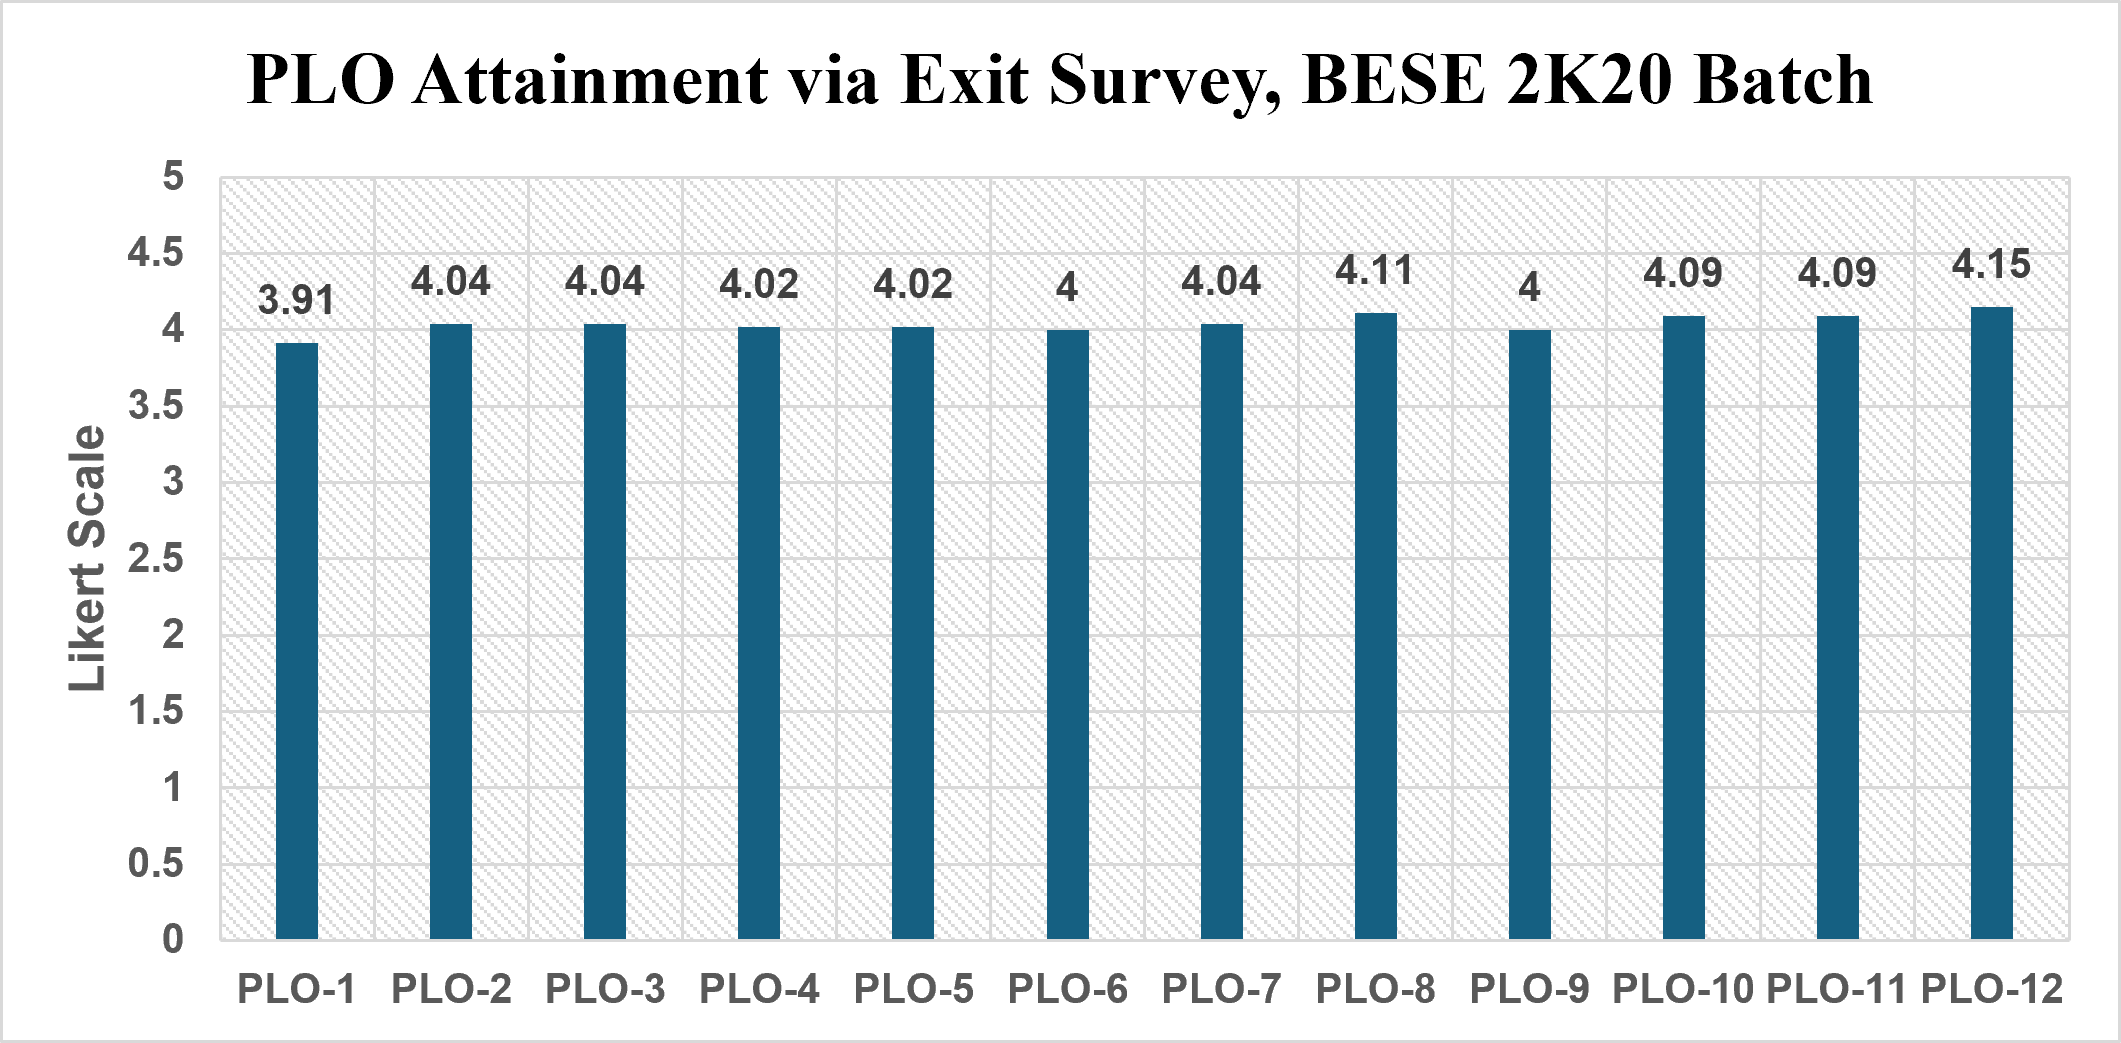
\includegraphics[width=0.90\textwidth]{images/criterion_2/media/image40.png}
\caption{PLO attainment based on the Graduate Exit Survey for the BESE 2K20 Batch.}
\label{fig:exit-survey-2k20}
\end{figure}

\begin{longtable}{>{\centering\arraybackslash}p{0.08\textwidth}
                  >{\raggedright\arraybackslash}p{0.74\textwidth}
                  >{\centering\arraybackslash}p{0.09\textwidth}}

\caption{Result of Exit Survey for the Batch 2K20}
\label{table:PLO attainment based on the Graduate Exit} \\

\toprule
\textbf{PLO} & \textbf{Question} & \textbf{Score} \\
\midrule
\endfirsthead

\multicolumn{3}{c}{\tablename\ \thetable{} -- continued from previous page} \\
\toprule
\textbf{PLO} & \textbf{Question} & \textbf{Score} \\
\midrule
\endhead

\midrule
\multicolumn{3}{r}{Continued on next page} \\
\endfoot

\bottomrule
\endlastfoot

PLO 1  & My engineering education has developed the knowledge and skills I will need for my future career. & 3.91 \\
PLO 2  & I can analyze engineering problems using fundamental principles of mathematics, science, and engineering. & 4.04 \\
PLO 3  & I have acquired the ability to analyze and develop solutions for complex, real-world engineering problems involving multiple constraints and stakeholders. & 4.04 \\
PLO 4  & I can independently design experiments, analyze and interpret data, and synthesize findings to draw valid conclusions. & 4.02 \\
PLO 5  & I can select and effectively use the latest tools employed in the engineering industry. & 4.02 \\
PLO 6  & I am able to assess societal, health, safety, legal and cultural implications and the consequent responsibilities relevant to professional engineering practices. & 4.00 \\
PLO 7  & I am able to understand the societal and environmental impacts of engineering solutions and recognize the importance of sustainable development. & 4.04 \\
PLO 8  & I consider ethical principles in my engineering practice and take responsibility for the outcomes of my decisions. & 4.11 \\
PLO 9  & I can work effectively both independently and as part of a team on projects that involve collaboration across diverse technical and non-technical fields. & 4.00 \\
PLO 10 & I can express technical concepts through reports, presentations, and discussions with both technical and non-technical audiences. & 4.09 \\
PLO 11 & I am able to apply engineering and management skills to contribute to or lead projects in multidisciplinary teams. & 4.09 \\
PLO 12 & I have the ability to recognize the importance of and pursue lifelong learning in the broader context of innovation and technological developments. & 4.15 \\

\end{longtable}

\subsection{Batch 2K21 Analysis}

The 2K21 batch showed a slight improvement in self-assessed confidence levels across core engineering competencies compared to 2K20, with scores spanning a range of \textbf{3.87 to 4.21} as shown in Figure~\ref{fig:exit-survey-2k21} and Table~\ref{table:exit-survey-2k21}.

\begin{itemize}
\item \textbf{Key Strengths:} Non-technical and professional attributes remained the strongest pillars. \textbf{Communication (PLO 10: 4.21)}, \textbf{Ethics (PLO 8: 4.20)}, and \textbf{Individual \& Team Work (PLO 9: 4.20)} were the top-rated outcomes.
\item \textbf{Areas of Relative Moderation:} \textbf{Modern Tool Usage (PLO 5: 3.87)} and \textbf{Engineering Knowledge (PLO 1: 3.99)} were the lowest across the dataset for this batch.
\end{itemize}

\begin{figure}[H]
\centering
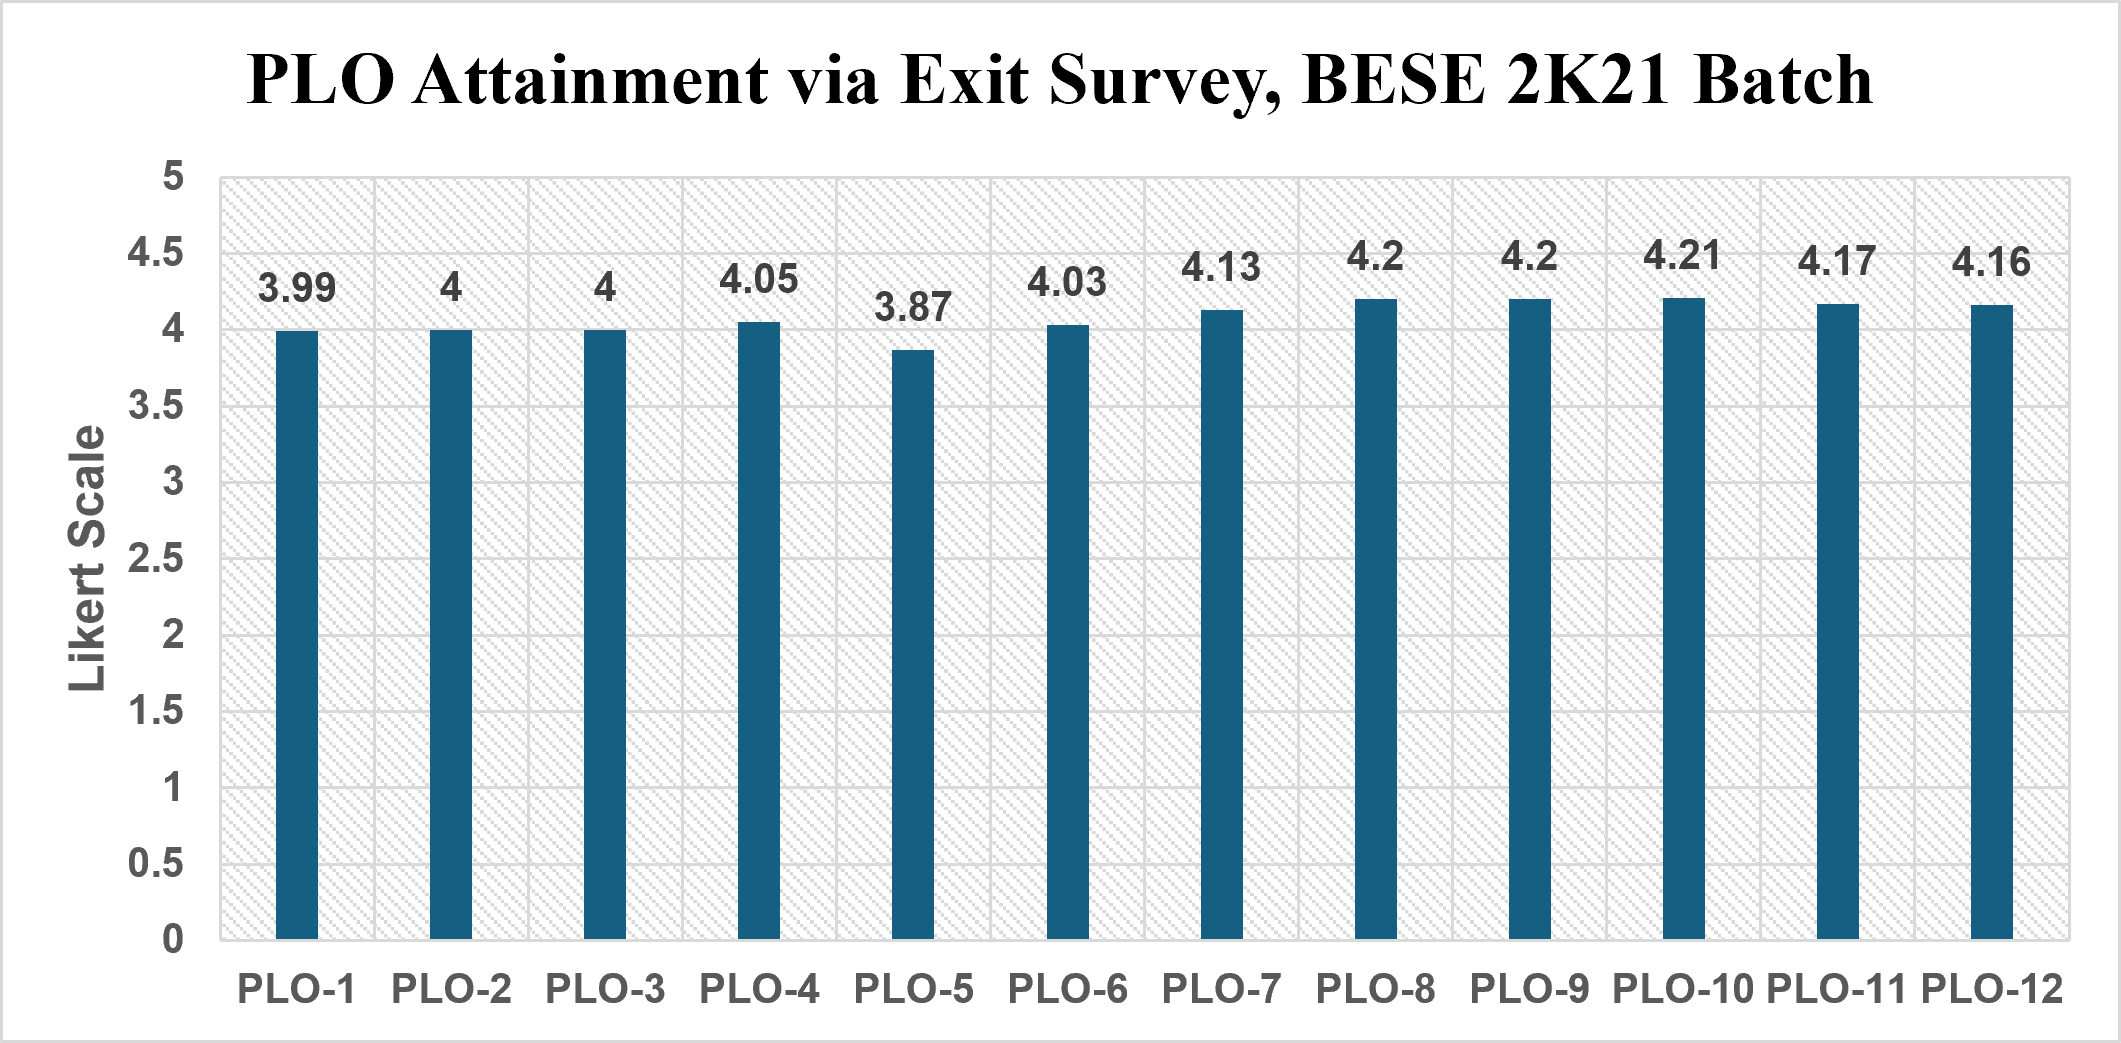
\includegraphics[width=0.90\textwidth]{images/criterion_2/media/image41.png}
\caption{PLO attainment based on the Graduate Exit Survey for the BESE 2K21 Batch.}
\label{fig:exit-survey-2k21}
\end{figure}


\begin{longtable}{>{\centering\arraybackslash}p{0.08\textwidth}
                  >{\raggedright\arraybackslash}p{0.74\textwidth}
                  >{\centering\arraybackslash}p{0.09\textwidth}}

\caption{Result of Exit Survey for the Batch 2K21}
\label{table:exit-survey-2k21} \\

\toprule
\textbf{PLO} & \textbf{Question} & \textbf{Score} \\
\midrule
\endfirsthead

\multicolumn{3}{c}{\tablename\ \thetable{} -- continued from previous page} \\
\toprule
\textbf{PLO} & \textbf{Question} & \textbf{Score} \\
\midrule
\endhead

\midrule
\multicolumn{3}{r}{Continued on next page} \\
\endfoot

\bottomrule
\endlastfoot

PLO 1  & My engineering education has developed the knowledge and skills I will need for my future career. & 3.99 \\
PLO 2  & I can analyze engineering problems using fundamental principles of mathematics, science, and engineering. & 4.00 \\
PLO 3  & I have acquired the ability to analyze and develop solutions for complex, real-world engineering problems involving multiple constraints and stakeholders. & 4.00 \\
PLO 4  & I can independently design experiments, analyze and interpret data, and synthesize findings to draw valid conclusions. & 4.05 \\
PLO 5  & I can select and effectively use the latest tools employed in the engineering industry. & 3.87 \\
PLO 6  & I am able to assess societal, health, safety, legal and cultural implications and the consequent responsibilities relevant to professional engineering practices. & 4.03 \\
PLO 7  & I am able to understand the societal and environmental impacts of engineering solutions and recognize the importance of sustainable development. & 4.13 \\
PLO 8  & I consider ethical principles in my engineering practice and take responsibility for the outcomes of my decisions. & 4.20 \\
PLO 9  & I can work effectively both independently and as part of a team on projects that involve collaboration across diverse technical and non-technical fields. & 4.20 \\
PLO 10 & I can express technical concepts through reports, presentations, and discussions with both technical and non-technical audiences. & 4.21 \\
PLO 11 & I am able to apply engineering and management skills to contribute to or lead projects in multidisciplinary teams. & 4.17 \\
PLO 12 & I have the ability to recognize the importance of and pursue lifelong learning in the broader context of innovation and technological developments. & 4.16 \\

\end{longtable}

\subsection{Batch 2K22 Analysis}

As shown in Figure~\ref{fig:exit-survey-2k22} and Table~\ref{table:exit-survey-2k22}, the scores for this 2K22 batch fall within a tight band from \textbf{3.89 to 4.07}, indicating a very honest, grounded, and realistic self-assessment by the graduating students.

\begin{itemize}
\item \textbf{Key Strengths:} The batch excels in interpersonal attributes, showcasing peak confidence in team collaboration across diverse fields (\textbf{PLO 9: 4.07}), effective technical communication (\textbf{PLO 10: 4.02}), and experimental design and data analysis (\textbf{PLO 4: 4.01}).
\item \textbf{Areas for Improvement:} Action is needed to reinforce professional ethics and accountability (\textbf{PLO 8: 3.89}), while incrementally boosting core engineering knowledge foundations (\textbf{PLO 1: 3.94}) and hands-on mastery of evolving industry toolsets (\textbf{PLO 5: 3.95}).
\end{itemize}


\begin{figure}[H]
\centering
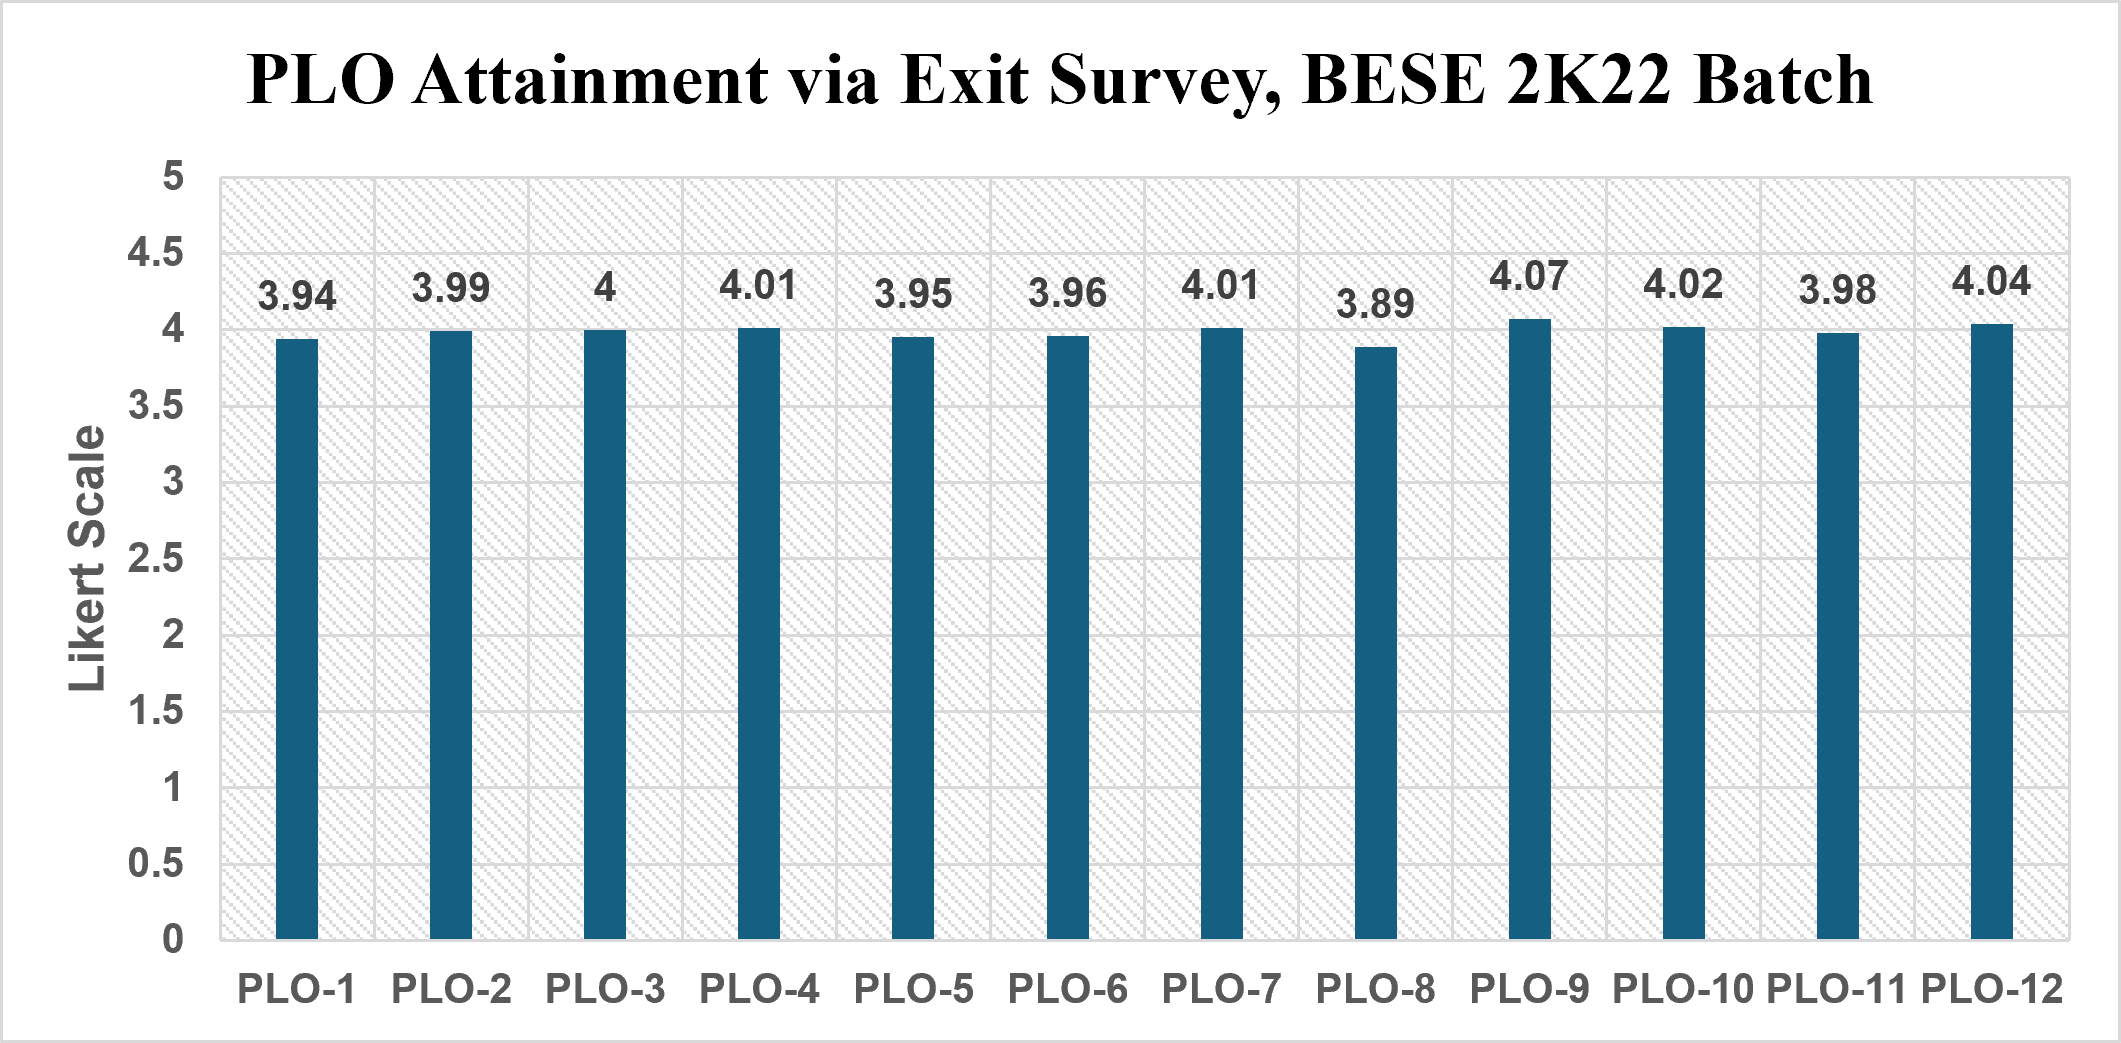
\includegraphics[width=0.90\textwidth]{images/criterion_2/media/image42.png}
\caption{PLO attainment based on the Graduate Exit Survey for the BESE 2K22 Batch.}
\label{fig:exit-survey-2k22}
\end{figure}

\begin{longtable}{>{\centering\arraybackslash}p{0.08\textwidth}
                  >{\raggedright\arraybackslash}p{0.74\textwidth}
                  >{\centering\arraybackslash}p{0.09\textwidth}}

\caption{Result of Exit Survey for the Batch 2K22}
\label{table:exit-survey-2k22} \\

\toprule
\textbf{PLO} & \textbf{Question} & \textbf{Score} \\
\midrule
\endfirsthead

\multicolumn{3}{c}{\tablename\ \thetable{} -- continued from previous page} \\
\toprule
\textbf{PLO} & \textbf{Question} & \textbf{Score} \\
\midrule
\endhead

\midrule
\multicolumn{3}{r}{Continued on next page} \\
\endfoot

\bottomrule
\endlastfoot

PLO 1  & My engineering education has developed the knowledge and skills I will need for my future career. & 3.94 \\
PLO 2  & I can analyze engineering problems using fundamental principles of mathematics, science, and engineering. & 3.99 \\
PLO 3  & I have acquired the ability to analyze and develop solutions for complex, real-world engineering problems involving multiple constraints and stakeholders. & 4.00 \\
PLO 4  & I can independently design experiments, analyze and interpret data, and synthesize findings to draw valid conclusions. & 4.01 \\
PLO 5  & I can select and effectively use the latest tools employed in the engineering industry. & 3.95 \\
PLO 6  & I am able to assess societal, health, safety, legal and cultural implications and the consequent responsibilities relevant to professional engineering practices. & 3.96 \\
PLO 7  & I am able to understand the societal and environmental impacts of engineering solutions and recognize the importance of sustainable development. & 4.01 \\
PLO 8  & I consider ethical principles in my engineering practice and take responsibility for the outcomes of my decisions. & 3.89 \\
PLO 9  & I can work effectively both independently and as part of a team on projects that involve collaboration across diverse technical and non-technical fields. & 4.07 \\
PLO 10 & I can express technical concepts through reports, presentations, and discussions with both technical and non-technical audiences. & 4.02 \\
PLO 11 & I am able to apply engineering and management skills to contribute to or lead projects in multidisciplinary teams. & 3.98 \\
PLO 12 & I have the ability to recognize the importance of and pursue lifelong learning in the broader context of innovation and technological developments. & 4.04 \\

\end{longtable}
\clearpage
\section{Corrective Action Form}
\label{annex:caf}

\begin{figure}[H]
\centering
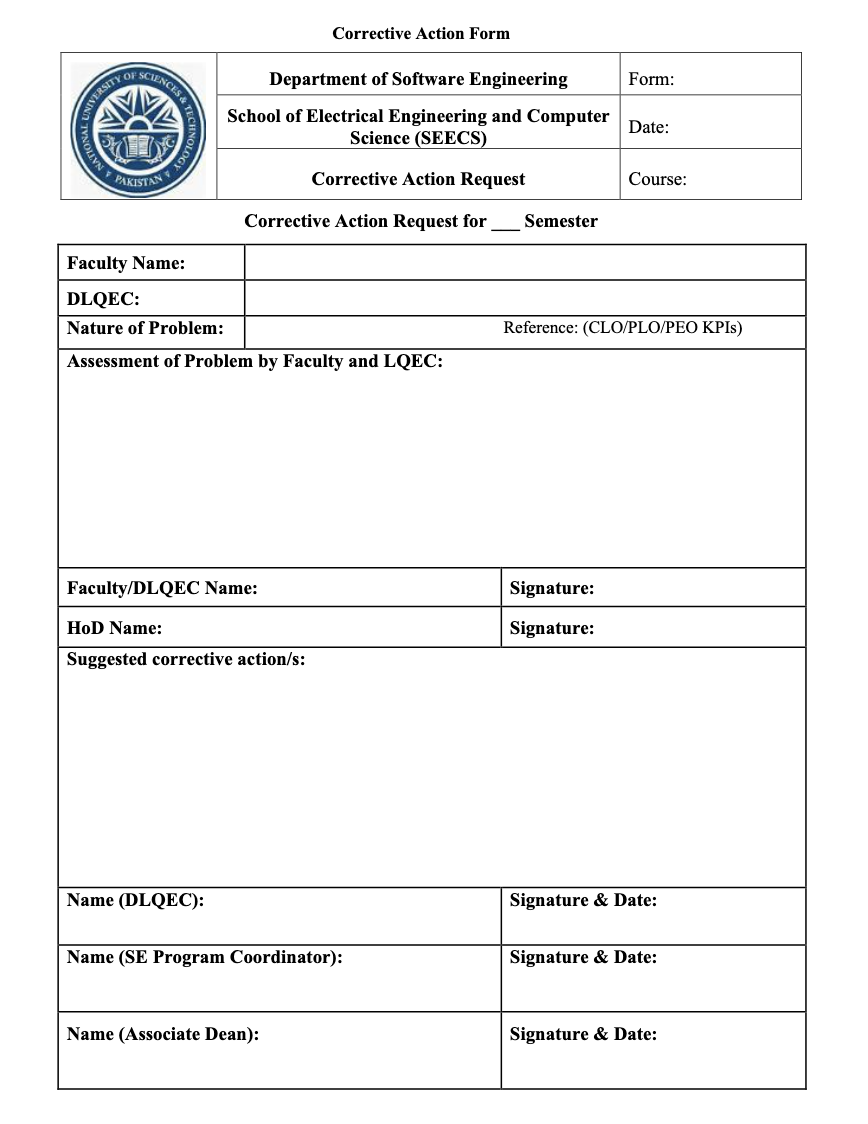
\includegraphics[width=1.0\textwidth]{images/criterion_2/media/corrective.png}
\caption{Corrective Action Form}
\end{figure}
%\includefullannexure{appendices/criterion_2/Corrective Action Form.pdf}

\section{Corrective Action Form  -- OOP}
\label{annex:caf-oop}
\includefullannexure{appendices/criterion_2/CAF_OOP.pdf}

\clearpage
\section{DBS Meeting Minutes}
\label{annex:dbs-mom}
%\includefullannexure{appendices/criterion_2/DBS Meeting Minutes.pdf}
\begin{figure}[H]
\centering
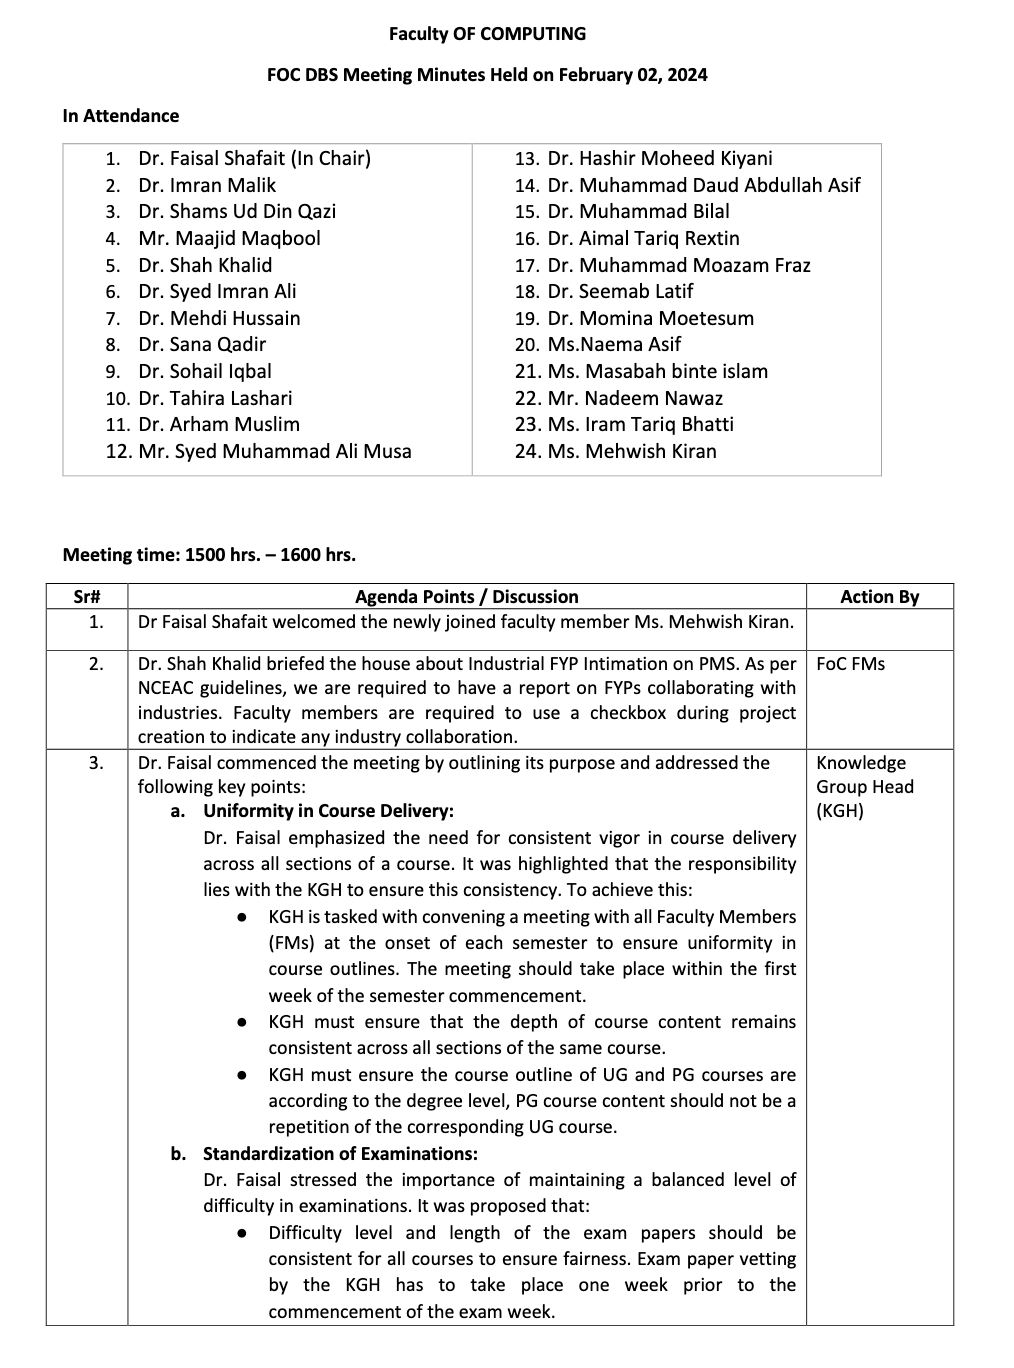
\includegraphics[width=1.0\textwidth]{images/criterion_2/media/dbs-min1.png}
\caption{DBS Meeting Minutes-2nd February 2024}
\end{figure}
\begin{figure}[H]
\centering
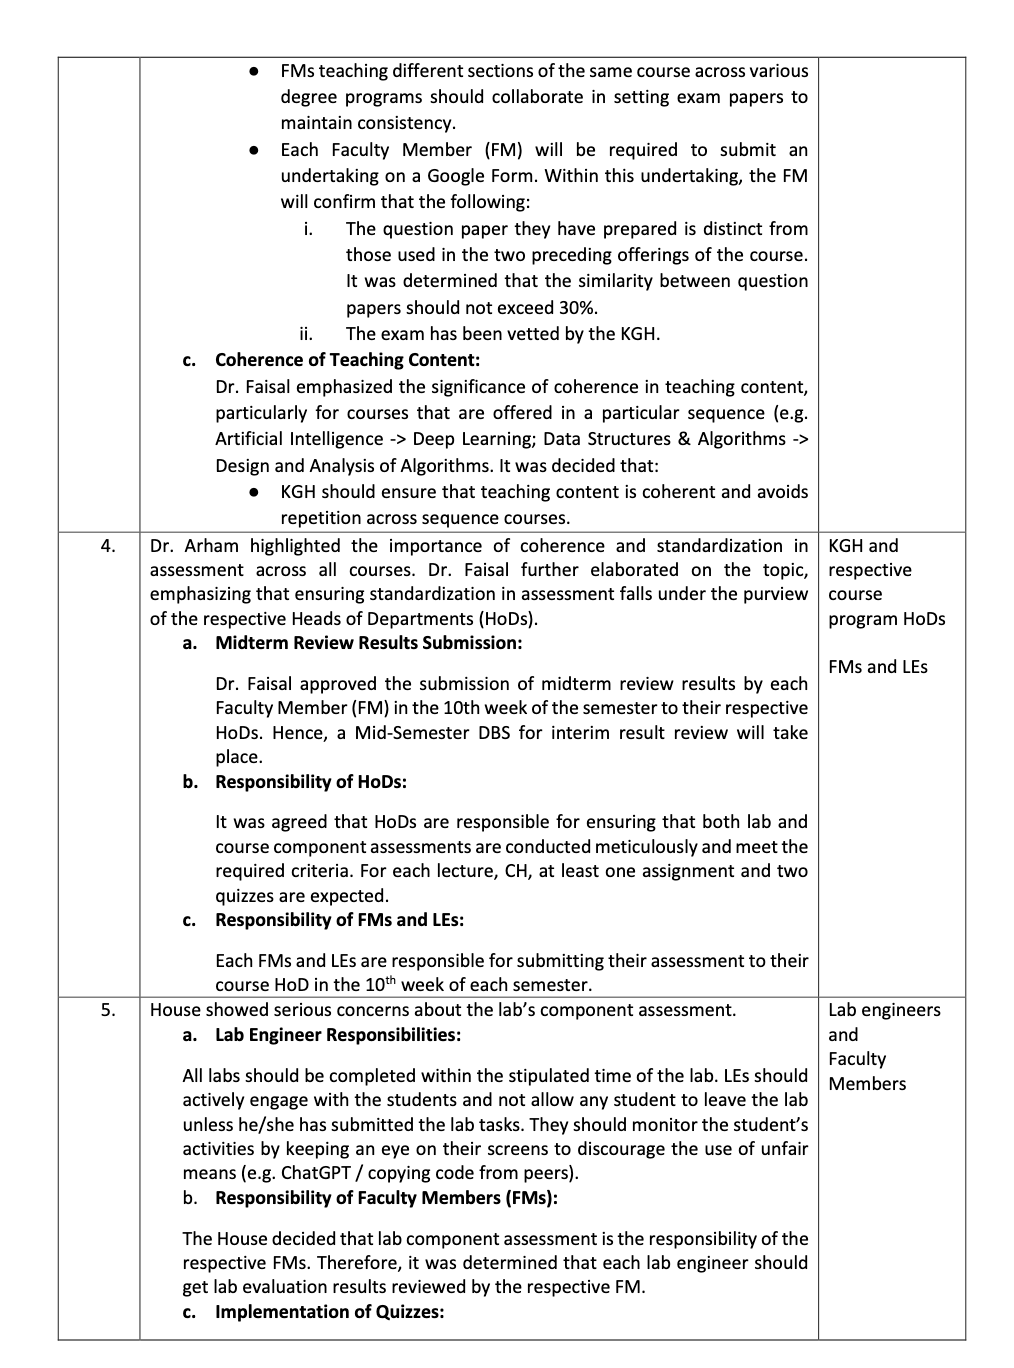
\includegraphics[width=1.0\textwidth]{images/criterion_2/media/dbs-min2.png}
\caption{DBS Meeting Minutes-2nd February 2024}
\end{figure}
\begin{figure}[H]
\centering
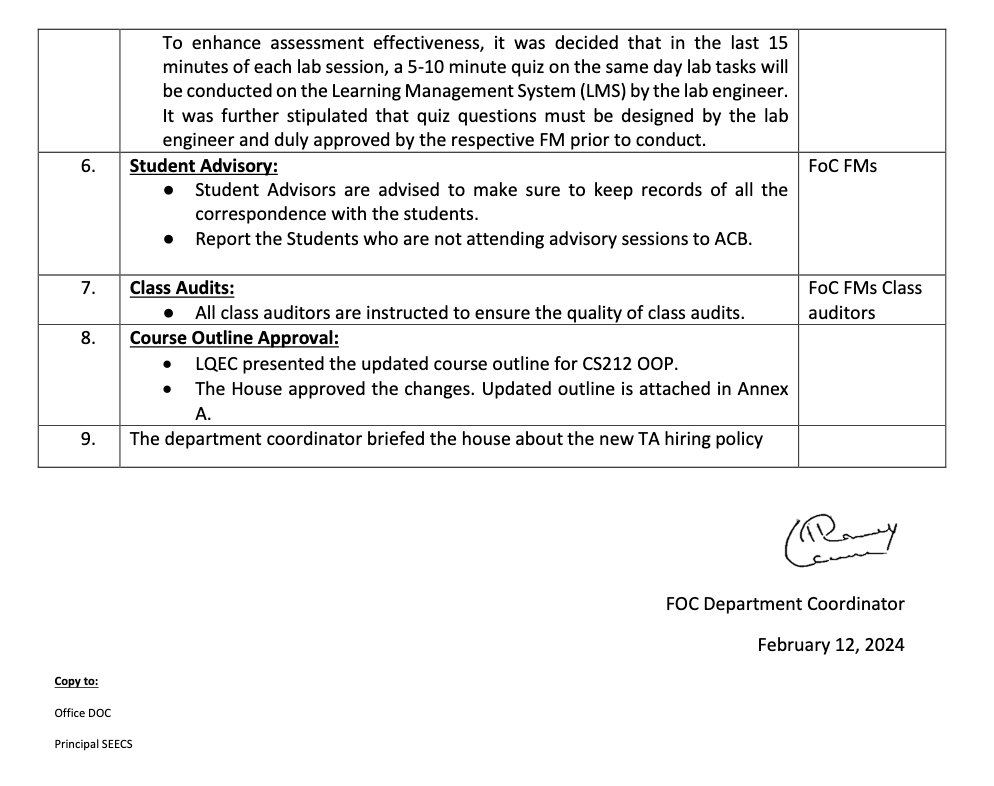
\includegraphics[width=1.0\textwidth]{images/criterion_2/media/dbs-min3.png}
\caption{DBS Meeting Minutes-2nd February 2024}
\end{figure}
\clearpage
\section{Counselling Form}
\label{annex:counselling-form}
\begin{figure}[H]
\centering
\fbox{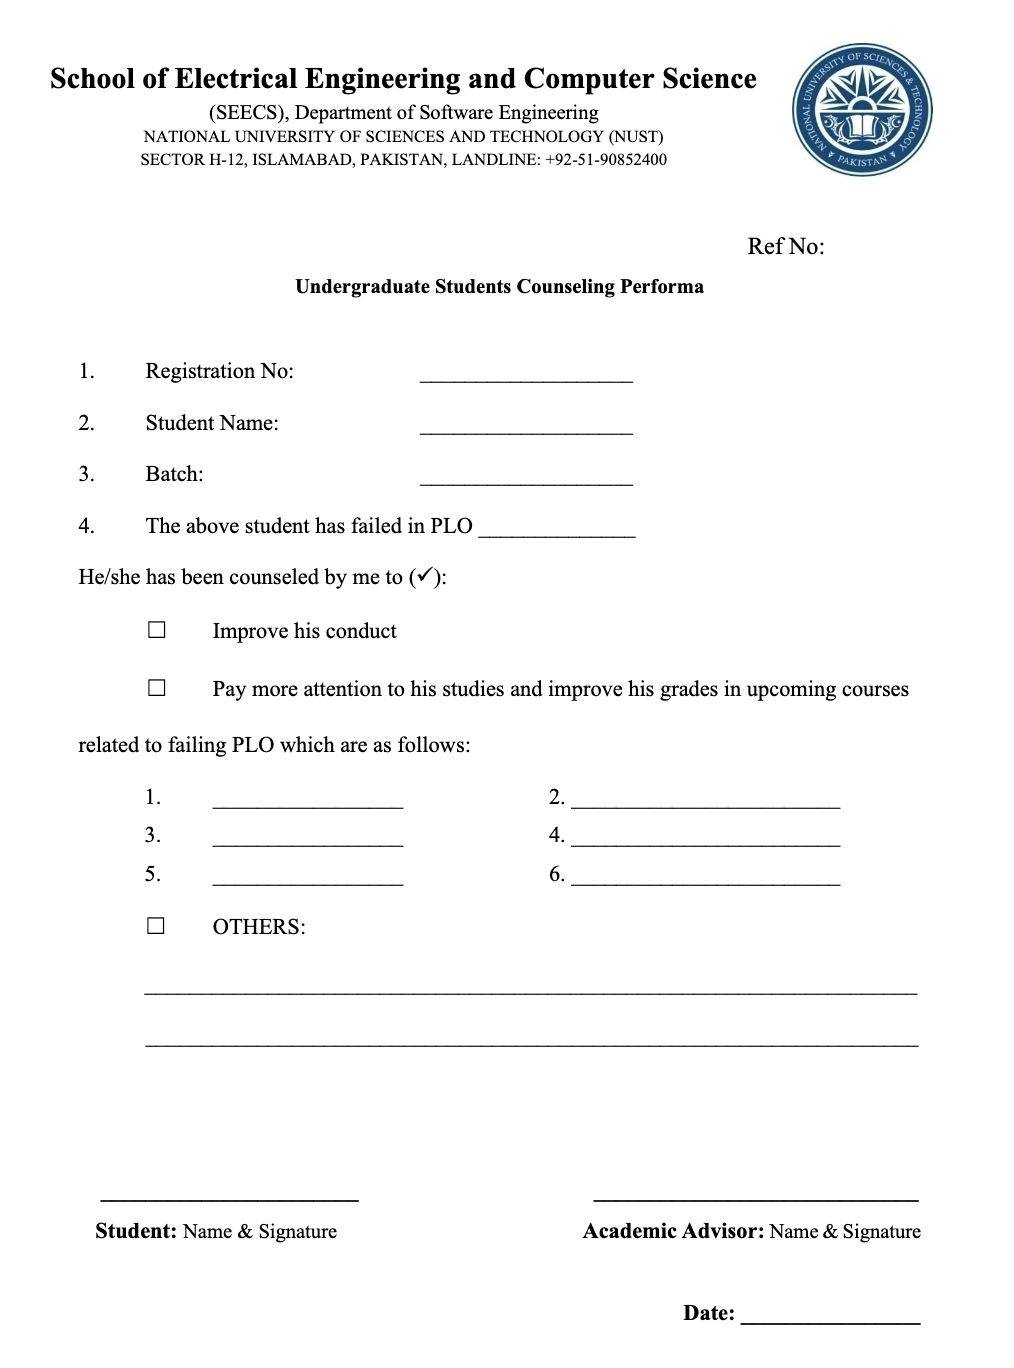
\includegraphics[width=1.0\textwidth]{images/criterion_2/media/council.png}}
\caption{Student Counseling Form}
\end{figure}
%\includefullannexure{appendices/criterion_2/Counselling Form.pdf}

\clearpage
\section{Warning Letter}
\label{annex:warning-letter}
\begin{figure}[H]
\centering
\fbox{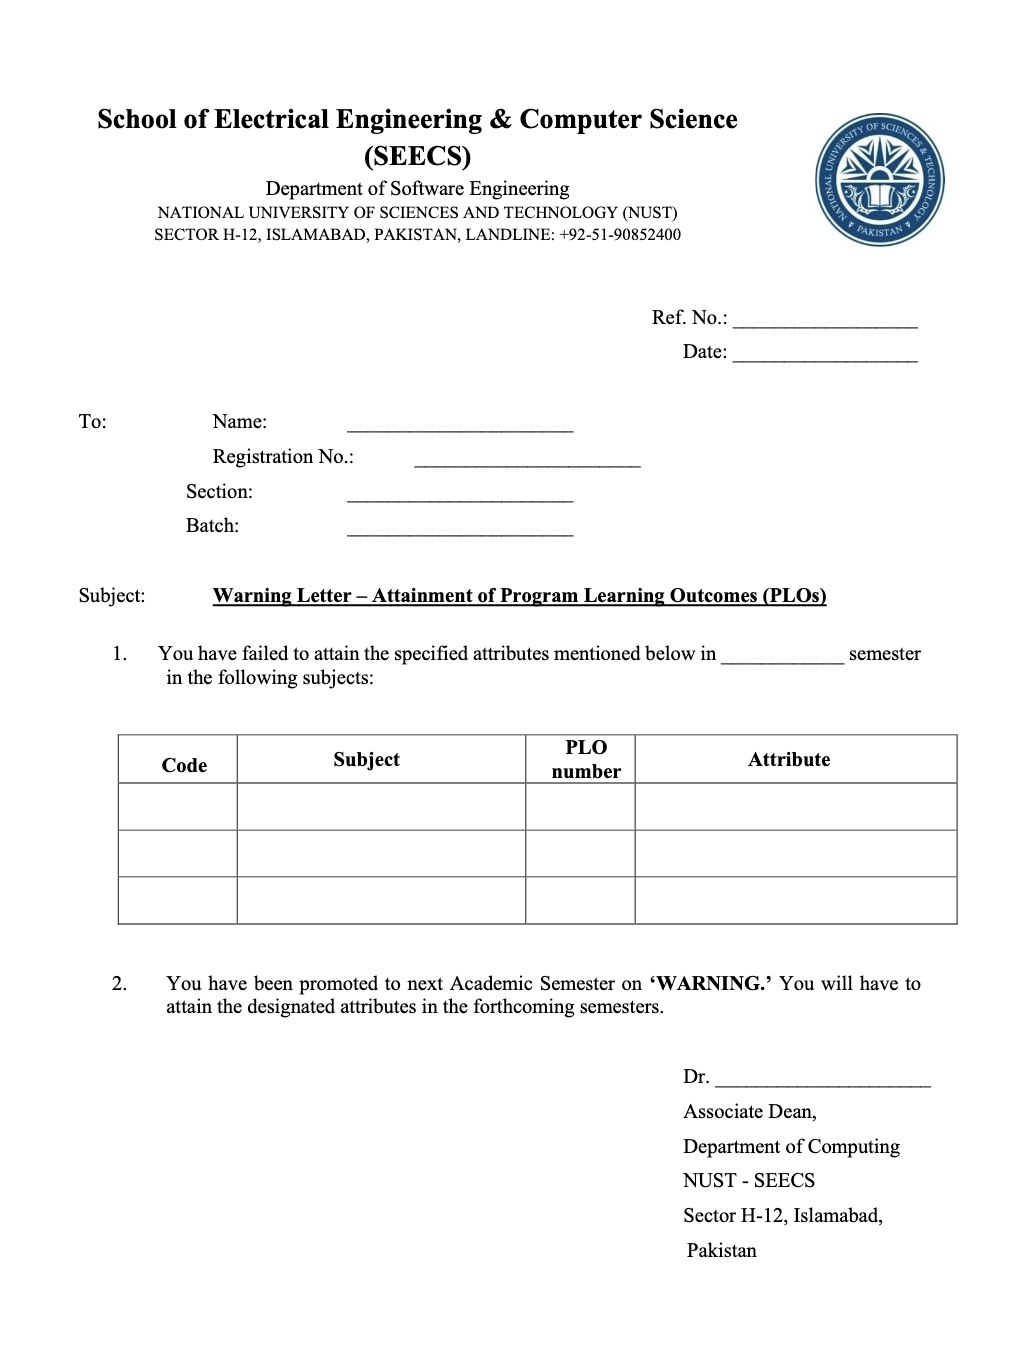
\includegraphics[width=1.0\textwidth]{images/criterion_2/media/warning.png}}
\caption{Sample Warning Letter}
\end{figure}
%\includefullannexure{appendices/criterion_2/Warning Letter.pdf}